% =====================================================================
% CAPÍTULO 6 — VERSIÓN FINAL DE LA REESTRUCTURACIÓN (ESQUELETO CON PLACEHOLDERS)

% Basado en indicaciones de la profesora guía (reunión, notas del alumno).
% Incluye ejemplos concretos de columnas para cada tabla, alineados con
% las columnas reales producidas por metrics.py / fairness.py /
% cross_dataset-2.py (bootstrap_metrics, evaluate_by_subgroup, etc.)
% =====================================================================

\chapter{Evaluación de Modelos Fundacionales}
\label{cap:evaluacion_modelos}

El Capítulo \ref{cap:seleccion_modelos} definió las tareas de evaluación y seleccionó los modelos fundacionales a comparar. El presente capítulo describe el protocolo experimental utilizado para evaluar el comportamiento de estos modelos frente a variaciones entre cohortes y subgrupos demográficos.

El protocolo se estructura en cuatro etapas: preprocesamiento de datos, extracción de representaciones visuales mediante los modelos fundacionales, entrenamiento de un clasificador sobre dichas representaciones, y evaluación cuantitativa mediante métricas de utilidad, equidad y generalización. Cada etapa se describe con el nivel de detalle necesario para garantizar la reproducibilidad del estudio.

La evaluación se centra en tres dimensiones complementarias. La primera dimensión corresponde a la utilidad predictiva global, medida mediante \textit{balanced accuracy}, \textit{macro-F1} y \textit{AUC}, complementada con la sensibilidad (\textit{recall}) por clase para identificar qué clases se detectan de forma confiable. La segunda dimensión analiza la equidad del rendimiento entre subgrupos demográficos, particularmente sexo y grupo de edad, mediante brechas de desempeño entre subgrupos. La tercera dimensión evalúa la generalización ante cambios de distribución, comparando el rendimiento en escenarios \textit{in-distribution} y \textit{out-of-distribution}. Estas tres dimensiones se evalúan de forma conjunta para cada combinación de tarea, modelo y clasificador, permitiendo una comparación sistemática del comportamiento de los modelos fundacionales en contextos clínicos diversos.

\section{preprocesamiento de datos}
\label{sec:preparacion_datos}

El preprocesamiento de las \textit{Whole Slide Images} (WSI) constituye la etapa previa indispensable a la extracción de representaciones mediante modelos fundacionales. Dado que las WSI pueden alcanzar dimensiones de varios gigapíxeles y tamaños de archivo de entre 1 y 8 GB, resulta computacionalmente inviable procesarlas de manera directa, lo que obliga a dividirlas en parches (\textit{patches}) de tamaño manejable para las arquitecturas basadas en \textit{Vision Transformers} (ViT). 

A continuación se describe el proceso de extracción de parches desde las WSI y los criterios de filtrado aplicados para descartar parches de baja calidad o sin información morfológica relevante. Ambas etapas se implementaron mediante un módulo de software desarrollado específicamente para este proyecto, \texttt{patch\_extractor}, cuyos parámetros de configuración se exploraron y validaron sobre cada conjunto de datos mediante un módulo de calibración complementario, \texttt{patch\_explorer}; la configuración final adoptada fue uniforme para todos los conjuntos de datos (Sección~\ref{sec:filtrado_parches}).

\subsection{Extracción de parches desde WSI}
\label{sec:extraccion_parches}

% Los parches se extrajeron de las WSI utilizando una estrategia de \textit{tiling} con parámetros fijos para todos los conjuntos de datos. Cada WSI se dividió en parches cuadrados de $224\times 224$ píxeles, obtenidos a una magnificación de 20$\times$. Esta resolución corresponde al tamaño de entrada estándar de los modelos fundacionales de patología computacional~\parencite{vorontsov2024virchow, chen2024uni}. La magnificación de 20$\times$ se seleccionó por corresponder a la resolución predominante en los conjuntos de datos utilizados en este estudio~\parencite{chen2024uni}. El desplazamiento (\textit{stride}) entre parches consecutivos fue igual al tamaño del parche (224 píxeles), lo que implica ausencia de solapamiento entre parches adyacentes.

La extracción de parches se realizó mediante un esquema de \textit{tiling} con ventana deslizante, en el cual cada WSI se recorre sistemáticamente generando parches cuadrados no superpuestos a una magnificación fija. El proceso considera tres etapas: (1) apertura de la WSI y determinación del nivel de la pirámide de resolución más cercano a la magnificación objetivo, (2) generación vectorizada de coordenadas de parches sobre la dimensión completa del \textit{slide}, y (3) lectura y extracción de cada parche en su resolución correspondiente.

\paragraph{Tamaño de parche} La elección de un tamaño de parche de $224\times224$ píxeles se justifica bajo el tamaño de entrada estándar utilizado por los \textit{encoders ViT} en la mayoría de los modelos fundacionales de patología digital publicados recientemente, por ejemplo UNI \parencite{chen2024uni} y Phikon-v2 \parencite{filiot2024phikonv2}, cuyos \textit{checkpoints} pre-entrenados fueron optimizados y validados con imágenes de esa resolución de entrada. Utilizar el mismo tamaño de parche que el empleado durante el pre-entrenamiento evita distorsiones por \textit{resize} adicional y maximiza la compatibilidad de la representación extraída con el dominio de entrenamiento original del modelo, un aspecto identificado como crítico en la literatura reciente sobre sensibilidad de modelos fundacionales a la escala de entrada.

\paragraph{Magnificación \textbf{$20\times$}} Esta se seleccionó por ser la magnificación óptica predominante reportada en los metadatos de adquisición de las cohortes utilizadas en este estudio, evitando así la necesidad de reescalados adicionales. Dado que los modelos fundacionales seleccionados en este trabajo fueron mayoritariamente pre-entrenados o validados a $20\times$, esta decisión minimiza el riesgo de una desalineación de dominio entre la escala de extracción y la escala de entrenamiento de los \textit{encoders}.

\paragraph{Formato de almacenamiento} Los parches extraídos se almacenaron en formato HDF5, organizados por WSI y agrupados dentro de un archivo por slide. Esta decisión responde a que HDF5 permite un acceso indexado eficiente a subconjuntos de parches sin necesidad de descomprimir archivos individuales, soporta compresión interna (se utilizó el esquema \texttt{lzf}, que prioriza velocidad de lectura/escritura sobre la tasa de compresión), y evita la sobrecarga del sistema de archivos asociada a almacenar potencialmente millones de archivos de imagen individuales por conjunto de datos, un problema documentado en pipelines de patología computacional a gran escala. Adicionalmente, el formato HDF5 permite escritura asíncrona mediante un hilo dedicado que libera a la GPU de esperar operaciones de disco.


La Tabla~\ref{tab:parametros_tiling} resume los parámetros utilizados en la extracción de parches. Estos valores se seleccionaron siguiendo las convenciones establecidas en la literatura de patología computacional, priorizando un equilibrio entre resolución espacial y eficiencia computacional.

\begin{table}[htbp]
    \centering
    \caption{Parámetros utilizados en la extracción de parches desde WSI.}
    \label{tab:parametros_tiling}
    \begin{tabular}{p{4cm} p{3cm} p{7cm}}
        \toprule
        \textbf{Parámetro} & \textbf{Valor} & \textbf{Justificación} \\
        \midrule
        Tamaño de parche & $224 \times 224$ px & Tamaño de entrada estándar en modelos fundacionales de patología digital pre-entrenados  \\
        Magnificación & $20\times$ & Magnificación predominante en las cohortes evaluadas \\
        Desplazamiento & $224$ px & Sin solapamiento; prioriza eficiencia computacional y de almacenamiento sobre cobertura redundante \\
        Formato de salida & HDF5 & Acceso indexado eficiente, compresión interna (\texttt{lzf}), evita sobrecarga de sistema de archivos por millones de imágenes individuales \\
        \bottomrule
    \end{tabular}
\end{table}

% La Figura~\ref{fig:tiling_ejemplo} ilustra el proceso de extracción de parches desde una WSI representativa. La estrategia de \textit{tiling} permite representar cada WSI como un conjunto discreto de parches de tamaño uniforme, lo que facilita el procesamiento posterior mediante los modelos fundacionales.

% \begin{figure}[htbp]
%     \centering
%     \fbox{\parbox{0.8\textwidth}{\centering Espacio para figura: proceso de extracción de parches desde WSI}}
%     \caption{Ilustración del proceso de extracción de parches. Se muestra una WSI original (izquierda), la segmentación de tejido (centro) y los parches extraídos (derecha).}
%     \label{fig:tiling_ejemplo}
% \end{figure}

\subsection{Filtrado de parches}
\label{sec:filtrado_parches}

Tras la extracción, se aplicó un proceso de filtrado destinado a descartar parches de baja calidad que podrían afectar negativamente la extracción de representaciones, ya sea por ausencia de tejido informativo o por artefactos de adquisición. Este filtrado se implementó mediante el módulo \texttt{patch\_extractor}, y sus parámetros se calibraron mediante el módulo exploratorio descrito a continuación; el valor final adoptado fue el mismo para todos los conjuntos de datos.

\paragraph{Estrategia de selección de parches} El módulo de filtrado opera sobre una miniatura (\textit{thumbnail}) de baja resolución de la WSI (512×512 o 1024×1024 píxeles, según configuración), evitando así el costo computacional de aplicar los criterios de filtrado sobre la imagen completa.


De esta forma, sobre la miniatura convertida a escala de grises, se calcula automáticamente un umbral óptimo mediante el método de Otsu, que maximiza la varianza entre clases (tejido/fondo) a partir del histograma de intensidades. A diferencia de un umbral fijo definido manualmente, el método de Otsu se adapta a la distribución de intensidades particular de cada imagen, lo que resulta más robusto frente a la variabilidad de tinción e iluminación entre cohortes. Los píxeles con intensidad de gris inferior al umbral de Otsu se clasifican como tejido. Prov-GigaPath aplica este método sobre imágenes reducidas para segmentar tejido, descartar regiones de fondo y seleccionar los \textit{tiles} que serán procesados posteriormente \parencite{xu2024provgigapath}.

Una vez generada la máscara binaria de tejido a nivel de miniatura, cada parche candidato (definido por sus coordenadas en la resolución completa de la WSI) se proyecta sobre la máscara y se calcula la fracción de píxeles de tejido contenida en su área mediante una tabla de suma acumulada, lo que permite evaluar todos los parches de una WSI en una única operación vectorizada de NumPy en lugar de iterar parche por parche. Los parches cuya fracción de tejido es inferior al umbral \texttt{tissue\_threshold} configurado se descartan.

En términos de los valores concretos utilizados, el umbral de tejido se fijó en 0.5 para todos los conjuntos de datos, en función de la proporción típica de tejido observada visualmente en las WSI de cada cohorte durante el proceso de calibración.

\paragraph{Módulo de exploración de parámetros} La calibración de ambos umbrales por conjunto de datos no se realizó de forma arbitraria, sino mediante un módulo de exploración de filtrado (\texttt{Filter Explorer}), implementado como una serie de notebooks reproducibles, que automatizan un flujo de cuatro pasos: (1) selección automática de la imagen más representativa del conjunto de datos, calculada como la distancia euclidiana normalizada entre las métricas descriptivas de cada imagen (porcentaje de tejido, porcentaje de hematoxilina/eosina, diversidad de color, brillo) y la mediana de dichas métricas sobre una muestra del conjunto de datos completo; (2) barrido sistemático de umbrales candidatos de \texttt{tissue\_threshold} (0.01 a 0.8) sobre la imagen representativa, cuantificando para cada umbral la cantidad de parches retenidos y descartados; (3) inspección visual de muestras de parches retenidos y descartados en el umbral elegido, permitiendo verificar cualitativamente que el criterio numérico se traduce en decisiones de filtrado sensatas (por ejemplo, que los parches retenidos efectivamente contienen morfología celular y los descartados corresponden a fondo o artefactos); y (4) exportación de la configuración final calibrada en formato YAML, lista para integrarse en el archivo de configuración del extractor de parches.

La Tabla~\ref{tab:impacto_filtrado} presenta el impacto del filtrado en la cantidad de parches por conjunto de datos. Se observa una reducción variable según el conjunto de datos, lo que refleja diferencias en la calidad de las WSI y en las condiciones de adquisición de las imágenes.

\begin{table}[htbp]
    \centering
    \caption{Impacto del filtrado de parches por conjunto de datos.}
    \label{tab:impacto_filtrado}
    \begin{tabular}{p{3.5cm} c c c}
        \toprule
        \textbf{Conjunto de datos} & \textbf{\# Parches totales} & \textbf{\# Parches válidos} & \textbf{Reducción (\%)} \\
        \midrule
        BCNB & 10.142.741 & 1.569.115 & 84.5\% \\
        HISTAI-Breast & 104.686.417 & 18.705.908 & 82.1\% \\
        HSI-BC & 16.279.898 & 3.392.893 & 79.2\% \\
        HISTAI-CRC-B1 & 242.948.021 & 45.787.518 & 81.2\% \\
        HISTAI-CRC-B2 & 4.828.511 & 816.171 & 83.1\% \\
        SurGen & 143.710.737 & 65.526.229 & 54.4\% \\
        \bottomrule
    \end{tabular}
\end{table}


\section{Extracción de representaciones}
\label{sec:extraccion_representaciones}

Una vez generado el conjunto de parches válidos, se
procedió a la extracción de representaciones visuales (\textit{embeddings})
mediante los modelos fundacionales seleccionados en el Capítulo~\ref{cap:seleccion_modelos}.
Este proceso se implementó en un script independiente,
\texttt{embed\_from\_patches\_opt}, diseñado específicamente para consumir los
archivos HDF5 de parches generados en la etapa de preprocesamiento y producir, para
cada combinación de conjunto de datos y modelo, un archivo HDF5 de embeddings a
nivel de parche.

Cada modelo fue utilizado como extractor de características congelado, es decir,
sin ajuste fino (\textit{fine-tuning}) de sus parámetros. Esta decisión se tomó con
el objetivo de evaluar directamente la calidad de las representaciones aprendidas
durante el preentrenamiento, sin introducir variaciones adicionales derivadas de la
adaptación a un dominio específico, siguiendo la práctica estándar de evaluación de
modelos fundacionales de patología digital mediante extracción de características
(\textit{feature extraction}).

\subsection{Protocolo de extracción de \textit{embeddings}}
\label{sec:protocolo-inferencia}

Los parches válidos, obtenidos en la etapa de preprocesamiento se almacenaron previamente en archivos HDF5 como tensores RGB de dimensiones 3×224×224, con valores enteros sin signo de 8 bits. Por ello, durante la extracción de representaciones no se aplicó un redimensionamiento adicional: cada parche se leyó directamente desde el archivo HDF5 y se procesó en lotes.

Para cada modelo fundacional, los valores de píxel se transfirieron a la GPU, se convirtieron a punto flotante y se reescalaron al intervalo [0,1]. Posteriormente, se aplicó la normalización asociada a cada encoder, utilizando las medias y desviaciones estándar definidas en el registro de modelos. Este procedimiento permitió mantener el preprocesamiento coherente con los requisitos de entrada de UNI2-h, Virchow2, Phikon-v2 y Prov-GigaPath. Cabe señalar que Prov-GigaPath fue pre-entrenado con parches de $256\times256$ píxeles~\parencite{xu2024provgigapath}, mientras que en este estudio todos los modelos se evaluaron con parches de $224\times224$; en consecuencia, las representaciones de Prov-GigaPath se obtienen a una resolución menor que la de su pre-entrenamiento, una diferencia metodológica que debe considerarse al comparar su desempeño con el de los demás encoders.

Los modelos se utilizaron exclusivamente como extractores de características congelados. Cada encoder se configuró en modo de evaluación y la generación de representaciones se ejecutó dentro de un contexto \texttt{torch.inference\_mode()}, evitando el cálculo y almacenamiento de gradientes. La dimensión final del embedding se determinó dinámicamente mediante una inferencia sobre una entrada sintética, lo que permitió adaptar automáticamente la escritura de los archivos de salida a cada arquitectura.

Para acelerar el procesamiento, se empleó una estrategia multi-GPU basada en procesos independientes. Cada proceso se asoció a una GPU, cargó los modelos requeridos bajo demanda y consumió tareas desde una cola compartida. Cada tarea correspondió a una combinación de slide y modelo fundacional. Los embeddings obtenidos se transfirieron a CPU en formato float32 y se almacenaron incrementalmente junto con las coordenadas espaciales de sus parches, conservando la correspondencia entre cada representación y su ubicación original en la WSI

\paragraph{Tamaño de lote (\textit{batch size}).}
El tamaño de lote empleado durante la extracción de embeddings no se mantuvo fijo
durante todo el desarrollo del proyecto, sino que se ajustó por razones de
eficiencia. En una primera etapa se utilizó un valor conservador de 32 parches
por lote, pensado para evitar problemas de memoria al trabajar con varios
conjuntos de datos. Sin embargo, según la disponibilidad de recursos en el servidor (GPUs disponibles)
el tamaño de los lotes varió entre 32 y 256. 

\subsection{Robustez y manejo de errores de E/S}
\label{sec:robustez-embeddings}

Dado que el procesamiento de cada conjunto de datos puede tomar varias horas, el
script incorpora mecanismos simples para tolerar fallos: reintentos automáticos
ante errores de lectura o escritura, un límite de reintentos por slide antes de
marcarlo como fallido, y la eliminación de cualquier archivo de salida que quede
incompleto por una interrupción. Al finalizar cada ejecución se genera además un
resumen (\texttt{embedding\_stats.csv}) con la cantidad de parches procesados y
los eventuales errores por slide, lo que facilita revisar que la extracción se
completó correctamente para todos los casos.

\subsection{Almacenamiento y verificación de embeddings}
\label{sec:almacenamiento-embeddings}

Las representaciones extraídas se almacenaron en archivos con extensión \texttt{.h5}
(formato HDF5), organizados jerárquicamente por conjunto de datos y modelo,
replicando la organización de directorios ya utilizada para los parches. 
Cada archivo contiene 
\textit{embeddings} de dimensiones $(N_{\text{parches}}, D)$, donde $N_{\text{parches}}$
corresponde al número total de parches válidos del slide y $D$ a la dimensión del
embedding reportada por cada modelo (Tabla~\ref{tab:modelos-embedding}), junto con
un \textit{dataset} \texttt{coords} que preserva la posición espacial de cada
parche dentro de la WSI de origen. Ambos \textit{datasets} se crean con tamaño
redimensionable (\texttt{maxshape=(None, D)}) y se escriben de forma incremental por
lotes, evitando mantener en memoria la totalidad de los \textit{embeddings} de un slide antes
de persistirlos en disco.

La verificación de integridad de los \textit{embeddings} generados incluyó: (1) confirmación
de que la dimensión del embedding coincide con la reportada por cada modelo en su
documentación oficial; (2) detección de valores faltantes (\texttt{NaN}) o
infinitos; y (3) validación de que cada paciente posea exactamente un \textit{embedding}
final tras la etapa de agregación. Los resultados de esta verificación se
registraron en archivos de log para trazabilidad.

La agregación de los \textit{embeddings} desde el nivel de parche hasta el nivel de
paciente se realizó en dos etapas de promedio aritmético: en primer lugar, los
embeddings de los $N_{\text{parches}}$ parches de cada WSI se promediaron para
obtener un único vector por \textit{slide}; en segundo lugar, los vectores de todas
las WSI de un mismo paciente se promediaron para producir el \textit{embedding} final
del paciente (dimensión $D$). De este modo, cada paciente queda representado por un
único vector independientemente del número de WSI y de parches disponibles.

La Tabla~\ref{tab:modelos-embedding} resume las características relevantes de cada
modelo fundacional utilizado en la etapa de extracción de representaciones.

\begin{table}[h]
\centering
\caption{Características de los modelos fundacionales utilizados para extracción de representaciones.}
\label{tab:modelos-embedding}
\begin{tabular}{lccc}
\hline
\textbf{Modelo} & \textbf{Arquitectura} & \textbf{Dim. embedding} & \textbf{Entrada} \\
\hline
UNI2-h        & ViT-H/14 & 1536 & 224$\times$224 \\
Virchow2      & ViT-H/14 & 2560 & 224$\times$224 \\
Phikon-v2     & ViT-L/16 & 1024 & 224$\times$224 \\
Prov-GigaPath & ViT-g/14 & 1536 & 224$\times$224 \\
\hline
\end{tabular}
\end{table}

En el resto del capítulo se utiliza la abreviatura \textit{UNI2} para referirse a UNI2-h."

\section{Diseño del clasificador y estrategia de evaluación}
\label{sec:diseno-clasificador}

La evaluación de los modelos fundacionales se implementó mediante un módulo
independiente, encargado de utilizar los embeddings extraídos previamente y
evaluarlos en las tareas definidas. De esta forma, el proceso de evaluación
se mantiene separado de las etapas de extracción de parches y generación de
representaciones.

El módulo recibe como entrada los embeddings asociados a cada paciente, junto
con su etiqueta correspondiente y los metadatos disponibles, tales como
dataset de origen, sexo y edad. A partir de esta información, se entrenan
clasificadores simples sobre las representaciones obtenidas desde cada modelo
fundacional. Finalmente, el módulo genera los resultados de desempeño global
y por subgrupos, los cuales son utilizados en el análisis posterior.

La implementación se organiza en dos etapas principales. En primer lugar, se
integran los metadatos de los pacientes con sus embeddings, generando un
archivo consolidado para cada combinación de tarea, modelo y conjunto de datos. Posteriormente,
este archivo se utiliza para entrenar los clasificadores, calcular las
métricas de evaluación y almacenar los resultados generados.

Esta organización permite ejecutar la evaluación de manera consistente para
las distintas tareas y modelos considerados. Además, facilita la
reproducibilidad de los experimentos, ya que cada combinación utiliza una
misma estructura de entrada y produce resultados comparables.

\subsection{Arquitectura del clasificador}
\label{sec:arquitectura_clasificador}

Se utilizó una red neuronal perceptrón multicapa (\texttt{MLPClassifier}) como clasificador. La arquitectura consiste en una capa oculta de 256 neuronas con función de activación ReLU, y el entrenamiento se limitó a un máximo de 500 iteraciones (\texttt{max\_iter=500}). La regularización se realizó mediante penalización L2 (\texttt{$\alpha=1e-4$}). Dado el desbalance de clases presente en varias tareas, las clases minoritarias del conjunto de entrenamiento se sobre-muestrearon con reposición hasta igualar el tamaño de la clase mayoritaria, lo que evita que el clasificador ignore las clases escasas. El \textit{early stopping}, con una fracción de validación interna del 10\,\%, se habilitó únicamente en las cohortes de menor tamaño (HSI-BC e HISTAI-CRC-B2) como regularización implícita frente al sobreajuste; en las cohortes grandes el entrenamiento se ejecutó por el número completo de iteraciones. Todos los entrenamientos usaron una semilla fija (\texttt{seed=42}).

El propósito de este clasificador no es construir un modelo clínico final,
sino utilizar una estrategia común para comparar la calidad de las
representaciones generadas por los distintos modelos fundacionales. De esta
forma, un mejor desempeño del clasificador sugiere que el embedding contiene
información más útil para resolver la tarea evaluada.

\subsection{Partición de datos}
\label{sec:particion_datos}

La estrategia de partición se adaptó al tamaño muestral de cada tarea, garantizando en todos los casos dos propiedades mediante \texttt{StratifiedGroupKFold}:

\begin{enumerate}
    \item \textbf{Estratificación por etiqueta}: la proporción de clases se preserva en cada partición, lo que es especialmente relevante en tareas con desbalance de clases.
    \item \textbf{Agrupación por paciente}: cada paciente aparece en una única partición, evitando fugas de información (\textit{data leakage}) entre entrenamiento y prueba. Esto es fundamental cuando un mismo paciente puede tener múltiples WSI asociadas.
\end{enumerate}

Para las tareas T1--T4 se empleó validación cruzada de $k=5$ pliegues (CV5). En cada iteración, el 80\,\% de los pacientes se destinó al entrenamiento y el 20\,\% restante a prueba, rotando el pliegue de prueba en cada iteración. Las métricas finales se reportan sobre las predicciones de prueba combinadas de los $k$ pliegues, y los intervalos de confianza al 95\,\% se calculan mediante \textit{bootstrap} no paramétrico a nivel de paciente sobre esas mismas predicciones, de modo que cada paciente contribuye exactamente una vez al conjunto de prueba. Este esquema maximiza el aprovechamiento de los datos y resulta esencial para disponer de tamaños de subgrupo suficientes en el análisis de equidad, especialmente en las cohortes pequeñas (p.\ ej., HSI-BC, $n=44$; HISTAI-CRC-B2, $n=46$--$57$).

Para la tarea T5-ORGAN, que integra las seis cohortes ($n=3675$), se empleó en cambio una partición fija en entrenamiento (70\,\%), validación (15\,\%) y prueba (15\,\%), suficiente para sostener un conjunto de prueba amplio ($n=525$) sin la complejidad adicional de la validación cruzada.

Todas las particiones se ejecutaron con una semilla fija (\texttt{seed=42}) para garantizar la reproducibilidad de los resultados. El conjunto de validación se utilizó exclusivamente para monitorear la convergencia del clasificador, mientras que el conjunto de prueba se reservó para la evaluación final.

\subsection{Esquema de evaluación}
\label{subsec:esquema-validacion}

Para cada combinación de modelo fundacional y tarea de clasificación, los
clasificadores se entrenaron utilizando los embeddings del conjunto de
entrenamiento. Posteriormente, se evaluó su desempeño sobre los conjuntos de
validación y prueba.

Los resultados del conjunto de prueba se utilizaron para reportar las
métricas finales de utilidad global, fairness por subgrupos e incertidumbre
estadística. Además de las
métricas generales, se generaron resultados separados según las variables
demográficas disponibles, particularmente sexo y grupo etario, cuando la
cantidad de datos permitió realizar dicho análisis.

Los resultados de cada ejecución se almacenaron en archivos estructurados,
incluyendo un resumen general de las métricas obtenidas y reportes detallados
por subgrupo. Esto permite comparar de manera sistemática el comportamiento
de los modelos en las distintas tareas, conjuntos de datos y grupos de
pacientes.

\section{Métricas de evaluación}
\label{sec:metricas_evaluacion}

La evaluación del comportamiento de los modelos fundacionales se realizó mediante un protocolo unificado que cubre tres dimensiones: utilidad predictiva global, equidad entre subgrupos demográficos y generalización ante cambios de distribución. A continuación se describen las métricas utilizadas en cada dimensión.

\subsection{Utilidad global}
\label{sec:utilidad_global}

La utilidad predictiva global se midió mediante tres métricas complementarias, cada una capturando un aspecto diferente del rendimiento del clasificador en escenarios con desbalance de clases:

\textbf{Balanced accuracy}. Corresponde a la media aritmética del \textit{recall} (sensibilidad) por clase:

\begin{equation}
    \text{BA} = \frac{1}{K} \sum_{k=1}^{K} \frac{TP_k}{TP_k + FN_k}
    \label{eq:balanced_accuracy}
\end{equation}

donde $K$ es el número de clases, $TP_k$ los verdaderos positivos y $FN_k$ los falsos negativos de la clase $k$. Esta métrica asigna igual peso a cada clase independientemente de su frecuencia, lo que la hace robusta al desbalance. Su valor varía entre 0 (rendimiento aleatorio uniforme) y 1 (clasificación perfecta). La balanced accuracy fue elegida como métrica principal de utilidad por su amplia adopción en evaluaciones de fairness en IA clínica~\parencite{tertytchny2024balanced}.

\textbf{Macro-F1}. Calcula el F1-score (media armónica de precisión y recall) por clase y luego promedia sin ponderar:

\begin{equation}
    \text{Macro-F1} = \frac{1}{K} \sum_{k=1}^{K} \frac{2 \cdot P_k \cdot R_k}{P_k + R_k}
    \label{eq:macro_f1}
\end{equation}

donde $P_k$ es la precisión y $R_k$ el recall de la clase $k$. A diferencia de la balanced accuracy, el macro-F1 penaliza tanto falsos positivos como falsos negativos, proporcionando una visión más completa del rendimiento. La complementariedad con la balanced accuracy permite detectar patrones de error distintos~\parencite{chen2023algorithmic}.

\textbf{Macro-AUC}. Corresponde al área bajo la curva ROC calculada mediante la estrategia one-vs-rest y promediada macro:

\begin{equation}
    \text{AUC}_{\text{OVR}} = \frac{1}{K} \sum_{k=1}^{K} \text{AUC}_k
    \label{eq:macro_auc}
\end{equation}

El AUC mide la capacidad de discriminación del clasificador independientemente del umbral de decisión, lo que la hace útil para comparar modelos en escenarios con distribuciones de clase desiguales. En tareas multiclase, la estrategia one-vs-rest calcula un AUC binario para cada clase contra todas las demás, y luego se promedia macro~\parencite{NEURIPS2024_c9826b9e}.

\textbf{Sensibilidad (recall) por clase}. Complementariamente a las métricas globales, se reporta la sensibilidad de cada clase, definida como la proporción de muestras de esa clase correctamente clasificadas:

\begin{equation}
    \text{Sens}_k = \frac{TP_k}{TP_k + FN_k}
    \label{eq:sensibilidad}
\end{equation}

donde $TP_k$ son los verdaderos positivos y $FN_k$ los falsos negativos de la clase $k$. La sensibilidad por clase permite identificar qué clases se detectan de forma confiable y cuáles quedan sistemáticamente omitidas, un aspecto relevante en contexto clínico donde un falso negativo puede tener consecuencias graves. Dado que la balanced accuracy (Ecuación~\ref{eq:balanced_accuracy}) corresponde a la media aritmética de estas sensibilidades, su desglose por clase no constituye una métrica global nueva, pero sí visibiliza la heterogeneidad que la BA promedia. Los intervalos de confianza al 95\,\% de cada sensibilidad se estimaron mediante bootstrap (percentiles 2,5 y 97,5) remuestreando pacientes con reposición, conforme al protocolo descrito en la Sección~\ref{sec:incertidumbre}.

\subsection{Fairness por subgrupos}
\label{sec:fairness_subgrupos}

La equidad entre subgrupos se evaluó mediante métricas de \textit{group fairness}, que cuantifican las diferencias de rendimiento entre grupos demográficos definidos por sexo y edad.

\textbf{Brecha de rendimiento entre subgrupos} (\textit{gap}). Se define como la diferencia máxima de rendimiento entre el subgrupo con mejor desempeño y el de peor desempeño:

\begin{equation}
    \Delta M = \max_{g \in G} M(g) - \min_{g \in G} M(g)
    \label{eq:gap}
\end{equation}

donde $M$ es la métrica de rendimiento (balanced accuracy o macro-F1) y $G$ el conjunto de subgrupos. Esta métrica se calcula tanto para balanced accuracy como para macro-F1, manteniendo coherencia con las métricas de utilidad global~\parencite{huang2025flex}.

\textbf{Brecha de AUC} (delta-AUC). Mide la diferencia máxima de AUC entre cualquier par de subgrupos:

\begin{equation}
    \Delta\text{AUC} = \max_{g \in G} \text{AUC}(g) - \min_{g \in G} \text{AUC}(g)
    \label{eq:delta_auc}
\end{equation}

Un valor elevado de delta-AUC indica que el modelo discrimina de forma desigual entre grupos demográficos, lo que constituye una forma de inequidad algorítmica~\parencite{obermeyer2019dissecting}.

\textbf{Equalized Odds}. Evalúa si las tasas de verdaderos positivos (\textit{TPR}) y falsos positivos (\textit{FPR}) son similares entre subgrupos:

\begin{align}
    \text{TPR gap} &= \max_{g \in G} \text{TPR}(g) - \min_{g \in G} \text{TPR}(g) \label{eq:tpr_gap} \\
    \text{FPR gap} &= \max_{g \in G} \text{FPR}(g) - \min_{g \in G} \text{FPR}(g) \label{eq:fpr_gap}
\end{align}

Equalized Odds requiere que tanto TPR como FPR sean similares entre grupos. Desviaciones de este criterio indican que el modelo tiene diferentes tasas de error para diferentes subgrupos~\parencite{chen2023algorithmic}. En tareas multiclase, el TPR y el FPR por subgrupo se definen como el promedio sobre clases del recall y del \textit{false positive rate} one-vs-rest, respectivamente; cuando todas las clases están presentes en el subgrupo, el TPR promedio coincide con la balanced accuracy del subgrupo (nota de las tablas de fairness del Apéndice~\ref{anexo:resultados_completos}). En este trabajo la brecha agregada de Equalized Odds no se reporta como métrica resumen: su extensión a escenarios multiclase requiere adaptaciones no triviales, y la información que sustenta esta métrica (TPR y FPR por subgrupo) se presenta directamente en las tablas de fairness del Apéndice~\ref{anexo:resultados_completos}~\parencite{matos2025critical}.

Los subgrupos evaluados fueron:

\begin{itemize}
    \item \textbf{Sexo}: masculino vs.\ femenino, cuando la variable estaba disponible en el conjunto de datos. En tareas de cáncer de mama, las cohortes son femeninas en su práctica totalidad (BCNB e HSI-BC exclusivamente femeninos; HISTAI-Breast con una fracción masculina marginal del 1,3\%), por lo que esta dimensión no se evaluó en dichas tareas.
    \item \textbf{Edad}: se utilizaron tres grupos de edad ($<50$, $50$--$70$ y $\geq 70$ años), basados en los rangos clínicamente relevantes para cáncer de mama~\parencite{lin2025fairpath} (premenopáusica, postmenopáusica estándar y adulto mayor). Los mismos cortes se aplicaron a las tareas colorrectales para mantener la comparabilidad entre tareas y con la literatura, aunque no derivan de una justificación clínica específica para ese dominio; esta es una limitación del análisis de equidad por edad en colorrectal.
\end{itemize}

Los subgrupos con menos de 10 pacientes se excluyeron del análisis de equidad: con tamaños inferiores, la balanced accuracy por subgrupo puede tomar un número muy reducido de valores posibles y los intervalos bootstrap resultan demasiado amplios o degenerados para sostener comparaciones entre grupos. Los resultados de equidad se reportan en las tablas de fairness del Apéndice~\ref{anexo:resultados_completos}; no se incluyen figuras dedicadas, dado que el número de combinaciones dataset-modelo-subgrupo es reducido y los valores con sus intervalos se aprecian directamente en las tablas.

En HISTAI-Breast, la cohorte analítica presenta un sesgo de selección hacia pacientes mayores: la mediana de edad se desplaza de 58 a 63 años al filtrar por la disponibilidad de biomarcadores (Sección~\ref{sec:trazabilidad_muestras}, Capítulo~\ref{cap:caracterizacion_datasets}). Este sesgo debe considerarse al interpretar las comparaciones por grupo etario de las tareas T1 y T2, donde el grupo $<$50 años es el menos representado.

\subsection{Generalización cross-dataset}
\label{sec:generalizacion}

La caída de rendimiento se cuantificó mediante la diferencia absoluta y relativa entre el rendimiento in-distribution (ID) y out-of-distribution (OOD):

\begin{align}
    \Delta_{\text{OOD}} &= M_{\text{ID}} - M_{\text{OOD}} \label{eq:delta_ood} \\
    \Delta_{\text{rel}} &= \frac{M_{\text{ID}} - M_{\text{OOD}}}{M_{\text{ID}}} \times 100\% \label{eq:delta_rel}
\end{align}

donde $M$ corresponde a la métrica de utilidad (balanced accuracy o macro-F1), el subíndice ID denota el rendimiento en el conjunto de prueba del mismo dataset de entrenamiento, y OOD denota el rendimiento en un dataset diferente al de entrenamiento.

Una caída elevada indica que el modelo aprendió representaciones específicas del sitio de entrenamiento que no se generalizan a otros centros o cohortes. Este fenómeno está ampliamente documentado en patología computacional~\parencite{huang2025flex, openmibood2025} y constituye una de las principales amenazas al despliegue clínico de modelos de IA.

Una consideración metodológica necesaria para interpretar estas cifras se refiere al número de clases efectivamente presentes en cada conjunto de prueba, ya que la balanced accuracy se calcula sobre las clases presentes en el conjunto evaluado. En las transferencias hacia HSI-BC, la cohorte solo contiene dos de las tres clases de HER2 (0/1+ y 3+), de modo que la evaluación OOD se realiza con un denominador $K=2$ frente al $K=3$ de la evaluación in-distribution; las caídas reportadas hacia esta cohorte combinan, por tanto, un cambio de distribución con un cambio de denominador, y los valores de BA-OOD inferiores al azar efectivo (0.5) indican desempeño peor que aleatorio en el problema binario reducido. En la dirección inversa, cuando HSI-BC actúa como fuente, la evaluación OOD se restringe a los pacientes de las clases compartidas ($n=575$ en BCNB y $n=320$ en HISTAI-Breast, Tabla~\ref{tab:anexo_her2_crossdataset}); los deltas negativos que se observan en esa dirección se discuten en la Sección~\ref{sec:resultado_her2}.

\subsection{Incertidumbre estadística}
\label{sec:incertidumbre}

Las métricas principales de utilidad (balanced accuracy y macro-F1), la sensibilidad por clase y las brechas derivadas ($\Delta$BA y $\Delta$OOD) se acompañaron de intervalos de confianza al 95\% calculados mediante bootstrap no paramétrico~\parencite{riley2025uncertainty}. El AUC y su brecha $\Delta$AUC se reportan como estimaciones puntuales: se incluyen como métricas complementarias de discriminación, mientras que las interpretaciones del capítulo se apoyan en la balanced accuracy y su incertidumbre. El procedimiento consiste en:

\begin{enumerate}
    \item Remuestrear con reemplazo el conjunto de prueba, obteniendo muestras del mismo tamaño que el original.
    \item Recalcular las métricas en cada muestra remuestreada.
    \item Repetir el proceso 1000 veces.
    \item Obtener los intervalos de confianza a partir de los percentiles 2.5 y 97.5 de la distribución bootstrap.
\end{enumerate}

El remuestreo se realizó a nivel de paciente, garantizando que todas las métricas se calculen sobre la misma estructura de datos que en la evaluación original. Esta estrategia es especialmente relevante en evaluaciones por subgrupos, donde los tamaños de muestra son más pequeños y la varianza de las métricas es mayor~\parencite{matos2025critical}.

Los intervalos de confianza permiten distinguir entre diferencias de rendimiento estadísticamente significativas y fluctuaciones debidas al azar. En particular, una brecha de fairness de 5 puntos en balanced accuracy puede ser estadísticamente indistinguible de cero en cohortes pequeñas, lo que subraya la importancia de reportar intervalos de confianza en lugar de estimaciones puntuales.


\section{Resultados}
\label{sec:resultados}

Los resultados se organizan por tarea de clasificación, siguiendo la nomenclatura definida en la Tabla~\ref{tab:nomenclatura_tareas}. Para cada tarea se presenta, en primer lugar, la distribución de clases de las cohortes analíticas y ejemplos representativos. Posteriormente, se reporta la utilidad predictiva de los modelos fundacionales, el análisis de equidad entre subgrupos demográficos cuando el tamaño muestral lo permite, y la evaluación de generalización entre conjuntos de datos.

La interpretación de los resultados considera de manera conjunta la \textit{balanced accuracy}, el macro-F1, el AUC, la sensibilidad por clase y sus intervalos de confianza. Las comparaciones entre tareas deben realizarse con cautela, dado que difieren en número de clases, prevalencia de las categorías, tamaño de las cohortes y disponibilidad de metadatos demográficos. En particular, una \textit{balanced accuracy} similar puede tener implicancias distintas en una tarea binaria y en una tarea multiclase con categorías escasas.

Las tablas numéricas completas de utilidad predictiva, sensibilidad por clase, equidad entre subgrupos y generalización cross-dataset se incluyen en el Apéndice~\ref{anexo:resultados_completos}. El cuerpo del capítulo prioriza las figuras y los hallazgos necesarios para interpretar el comportamiento comparativo de los modelos y las limitaciones de cada cohorte.

\begin{table}[htbp]
\centering
\caption{Nomenclatura utilizada para referenciar cada tarea de clasificación a lo largo del capítulo.}
\label{tab:nomenclatura_tareas}
\begin{tabular}{l l l l}
\toprule
\textbf{Código} & \textbf{Tarea} & \textbf{Dominio} & \textbf{\# Clases} \\
\midrule
T1-HER2   & Estado HER2               & Mama         & 3 \\
T2-MOLSUB & Subtipo molecular         & Mama         & 4 \\
T3-SITE   & Sitio anatómico           & Colorrectal  & 9 \\
T4-SIDE   & Lateralidad               & Colorrectal  & 5 \\
T5-ORGAN  & Clasificación de órgano   & Mama + CRC   & 2 \\
\bottomrule
\end{tabular}
\end{table}

% ---------------------------------------------------------------------
% TABLA "SEMÁFORO" -- cuerpo principal

% Columnas: Tarea | Dataset | BA_UNI2 | BA_Virchow2 | BA_Phikonv2 | BA_ProvGigaPath
% Fuente: balanced_accuracy (point estimate) de bootstrap_metrics() por
% combinación (task, dataset, model). Color = f(BA, K_clases) vs. azar 1/K.
% ---------------------------------------------------------------------
% \begin{table}[htbp]
% \centering
% \caption{Panorama general de desempeño (balanced accuracy) por tarea, dataset y modelo. Color según la ganancia normalizada sobre el azar, $z = (BA - 1/K)/(1 - 1/K)$, con $K$ el número de clases presentes en la cohorte: verde si $z \geq 0.30$; amarillo si $0.10 \leq z < 0.30$; rojo si $z < 0.10$. Detalle con IC 95\% en Apéndice~\ref{anexo:resultados_completos}.}
% \label{tab:panorama_semaforo}
% \begin{tabular}{l l c c c c}
% \toprule
% \textbf{Tarea} & \textbf{Dataset} & \textbf{UNI2} & \textbf{Virchow2} & \textbf{Phikon-v2} & \textbf{Prov-GigaPath} \\
% \midrule
% T1-HER2   & BCNB          & \cellcolor{yellow!40}0.46 & \cellcolor{yellow!40}0.43 & \cellcolor{yellow!40}0.42 & \cellcolor{yellow!40}0.45 \\
% T1-HER2   & HISTAI-Breast & \cellcolor{red!30}0.36    & \cellcolor{red!30}0.37    & \cellcolor{red!30}0.38    & \cellcolor{red!30}0.38 \\
% T1-HER2   & HSI-BC        & \cellcolor{red!30}0.44    & \cellcolor{red!30}0.42    & \cellcolor{red!30}0.28    & \cellcolor{yellow!40}0.56 \\
% T2-MOLSUB & BCNB          & \cellcolor{green!25}0.48  & \cellcolor{yellow!40}0.43 & \cellcolor{yellow!40}0.43 & \cellcolor{yellow!40}0.47 \\
% T2-MOLSUB & HISTAI-Breast & \cellcolor{yellow!40}0.36 & \cellcolor{yellow!40}0.35 & \cellcolor{yellow!40}0.33 & \cellcolor{yellow!40}0.34 \\
% T2-MOLSUB & HSI-BC        & \cellcolor{red!30}0.32    & \cellcolor{red!30}0.17    & \cellcolor{red!30}0.22    & \cellcolor{yellow!40}0.33 \\
% T3-SITE   & HISTAI-CRC-B1 & \cellcolor{yellow!40}0.20 & \cellcolor{yellow!40}0.21 & \cellcolor{yellow!40}0.21 & \cellcolor{yellow!40}0.21 \\
% T3-SITE   & HISTAI-CRC-B2 & \cellcolor{red!30}0.12    & \cellcolor{red!30}0.14    & \cellcolor{red!30}0.09    & \cellcolor{red!30}0.13 \\
% T3-SITE   & SurGen        & \cellcolor{yellow!40}0.37 & \cellcolor{yellow!40}0.31 & \cellcolor{yellow!40}0.32 & \cellcolor{yellow!40}0.32 \\
% T4-SIDE   & HISTAI-CRC-B1 & \cellcolor{yellow!40}0.33 & \cellcolor{yellow!40}0.32 & \cellcolor{yellow!40}0.29 & \cellcolor{yellow!40}0.33 \\
% T4-SIDE   & HISTAI-CRC-B2 & \cellcolor{red!30}0.12    & \cellcolor{red!30}0.17    & \cellcolor{red!30}0.12    & \cellcolor{red!30}0.16 \\
% T4-SIDE   & SurGen        & \cellcolor{yellow!40}0.37 & \cellcolor{yellow!40}0.34 & \cellcolor{yellow!40}0.32 & \cellcolor{yellow!40}0.32 \\
% T5-ORGAN  & Combinado     & \cellcolor{green!25}1.00  & \cellcolor{green!25}1.00  & \cellcolor{green!25}1.00  & \cellcolor{green!25}1.00 \\
% \bottomrule
% \end{tabular}
% \end{table}

% =====================================================================
% 6.1 -- SUBSECCIÓN POR TAREA (repetir estructura para T1..T5)
% =====================================================================

\subsection{T1: Estado HER2}
\label{sec:resultado_her2}

\subsubsection{Descripción de la tarea y distribución de clases}

La tarea T1-HER2 consiste en clasificar el estado del receptor HER2 del cáncer de mama en tres categorías: negativo (0/1+), equívoco (2+) y positivo (3+), a partir de la expresión detectada por inmunohistoquímica. En BCNB ($n=1058$) la clase 2+ concentra el 45.7\,\% de los casos, seguida de 0/1+ (34.9\,\%) y 3+ (19.5\,\%); en HISTAI-Breast ($n=870$) la clase 2+ es aún más predominante (63.2\,\%), mientras que en HSI-BC ($n=44$) solo están representadas las clases 0/1+ (81.8\,\%) y 3+ (18.2\,\%), sin casos de 2+. La Figura~\ref{fig:dist_her2} muestra la distribución de clases por conjunto de datos y la Figura~\ref{fig:ejemplos_her2} ejemplos representativos de parches para cada clase.

\begin{figure}[htbp]
\centering
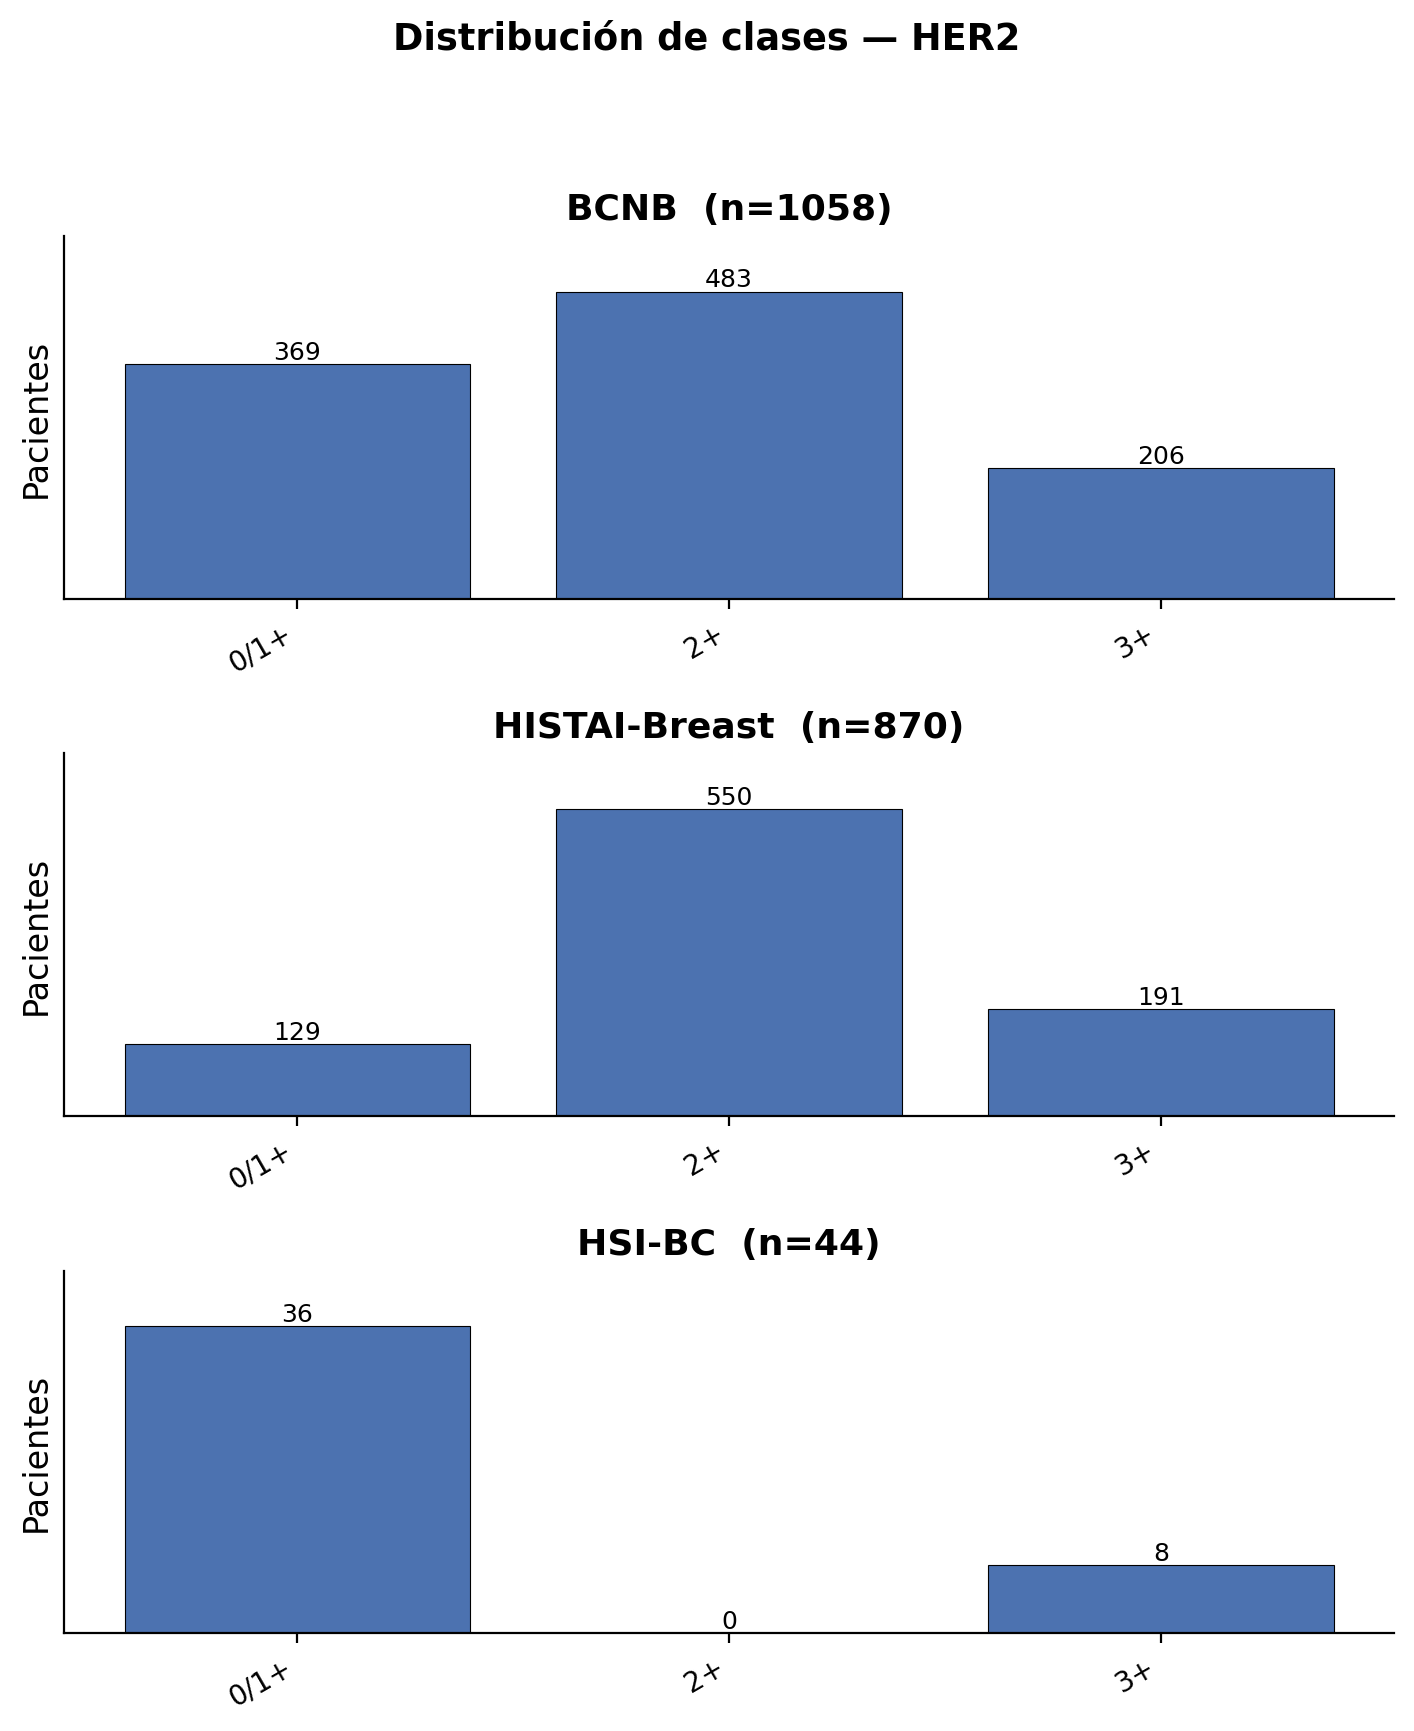
\includegraphics[width=0.5\textwidth]{figures/distribucion_clases/her2}
\caption{Distribución de clases de la tarea HER2 por conjunto de datos.}
\label{fig:dist_her2}
\end{figure}

\subsubsection{Desempeño por modelo y dataset}

% En BCNB las balanced accuracy oscilan entre 0.418 (Phikon-v2) y 0.455 (UNI2), con AUC entre 0.602 y 0.632: todos los modelos superan el azar (0.333), pero con un margen modesto. En HISTAI-Breast el desempeño desciende a 0.364--0.381, apenas por encima del azar, y en HSI-BC, donde el azar efectivo es 0.5 al estar presentes solo dos clases, UNI2 (0.438), Virchow2 (0.417) y Phikon-v2 (0.278) quedan por debajo de él, mientras que Prov-GigaPath alcanza 0.562 [0.359, 0.762] (Figura~\ref{fig:ba_her2}). El AUC es coherente con este patrón: sobre HSI-BC, UNI2 (0.389) y Phikon-v2 (0.184) presentan valores por debajo del azar, lo que, dado el reducido tamaño de la cohorte, indica ausencia de señal aprendida o ruido muestral extremo. El desglose por clase muestra que la clase 2+ es la mejor detectada en las cohortes grandes (sensibilidad 0.573--0.625 en BCNB y 0.709--0.747 en HISTAI-Breast), en línea con su condición de clase mayoritaria (45.7\,\% y 63.2\,\% de los casos, respectivamente), en tanto que 0/1+ y 3+ se detectan de forma deficiente (0.140--0.403); en HSI-BC, Phikon-v2 y Virchow2 no detectan ningún caso 3+ (sensibilidad 0.000).

En BCNB, la \textit{balanced accuracy} oscila entre 0.418 para Phikon-v2 y 0.455 para UNI2, mientras que el AUC macro varía entre 0.602 y 0.632. Por tanto, todos los modelos superan el nivel de referencia de 0.333 correspondiente a tres clases, aunque con una ganancia limitada. En HISTAI-Breast, la \textit{balanced accuracy} disminuye al intervalo de 0.364 a 0.381, también cercano al nivel de referencia. En HSI-BC, donde solo están presentes dos clases y el nivel de referencia es 0.5, UNI2, Virchow2 y Phikon-v2 obtienen valores inferiores a dicho nivel, mientras que Prov-GigaPath alcanza 0.562 con un IC 95\% de [0.359, 0.762]. La amplitud de este último intervalo, junto con el tamaño de cohorte de $n=44$, impide establecer una diferencia concluyente respecto del nivel de referencia.

El AUC macro sigue un patrón similar. En HSI-BC, UNI2 y Phikon-v2 alcanzan valores inferiores a 0.5, de 0.389 y 0.184, respectivamente. Dado el tamaño reducido de esta cohorte y la ausencia de intervalos de confianza para AUC, estos resultados deben interpretarse como evidencia descriptiva de inestabilidad y baja discriminación, no como una estimación precisa del desempeño poblacional.

El análisis por clase muestra una marcada heterogeneidad. En BCNB, la sensibilidad de la categoría 2+ se encuentra entre 0.573 y 0.625, mientras que en HISTAI-Breast varía entre 0.709 y 0.747. Las categorías 0/1+ y 3+ presentan sensibilidades más bajas, entre 0.140 y 0.403 en las cohortes grandes. La mayor sensibilidad de la categoría 2+ coincide con su mayor prevalencia en ambos datasets, lo que es compatible con una influencia del desbalance de clases; sin embargo, estos resultados no permiten atribuir causalmente la diferencia de sensibilidad a la frecuencia de la categoría. En HSI-BC, Virchow2 y Phikon-v2 no identifican ningún caso de la categoría 3+, aunque esta observación se basa en un número reducido de pacientes.

\begin{figure}[htbp]
\centering
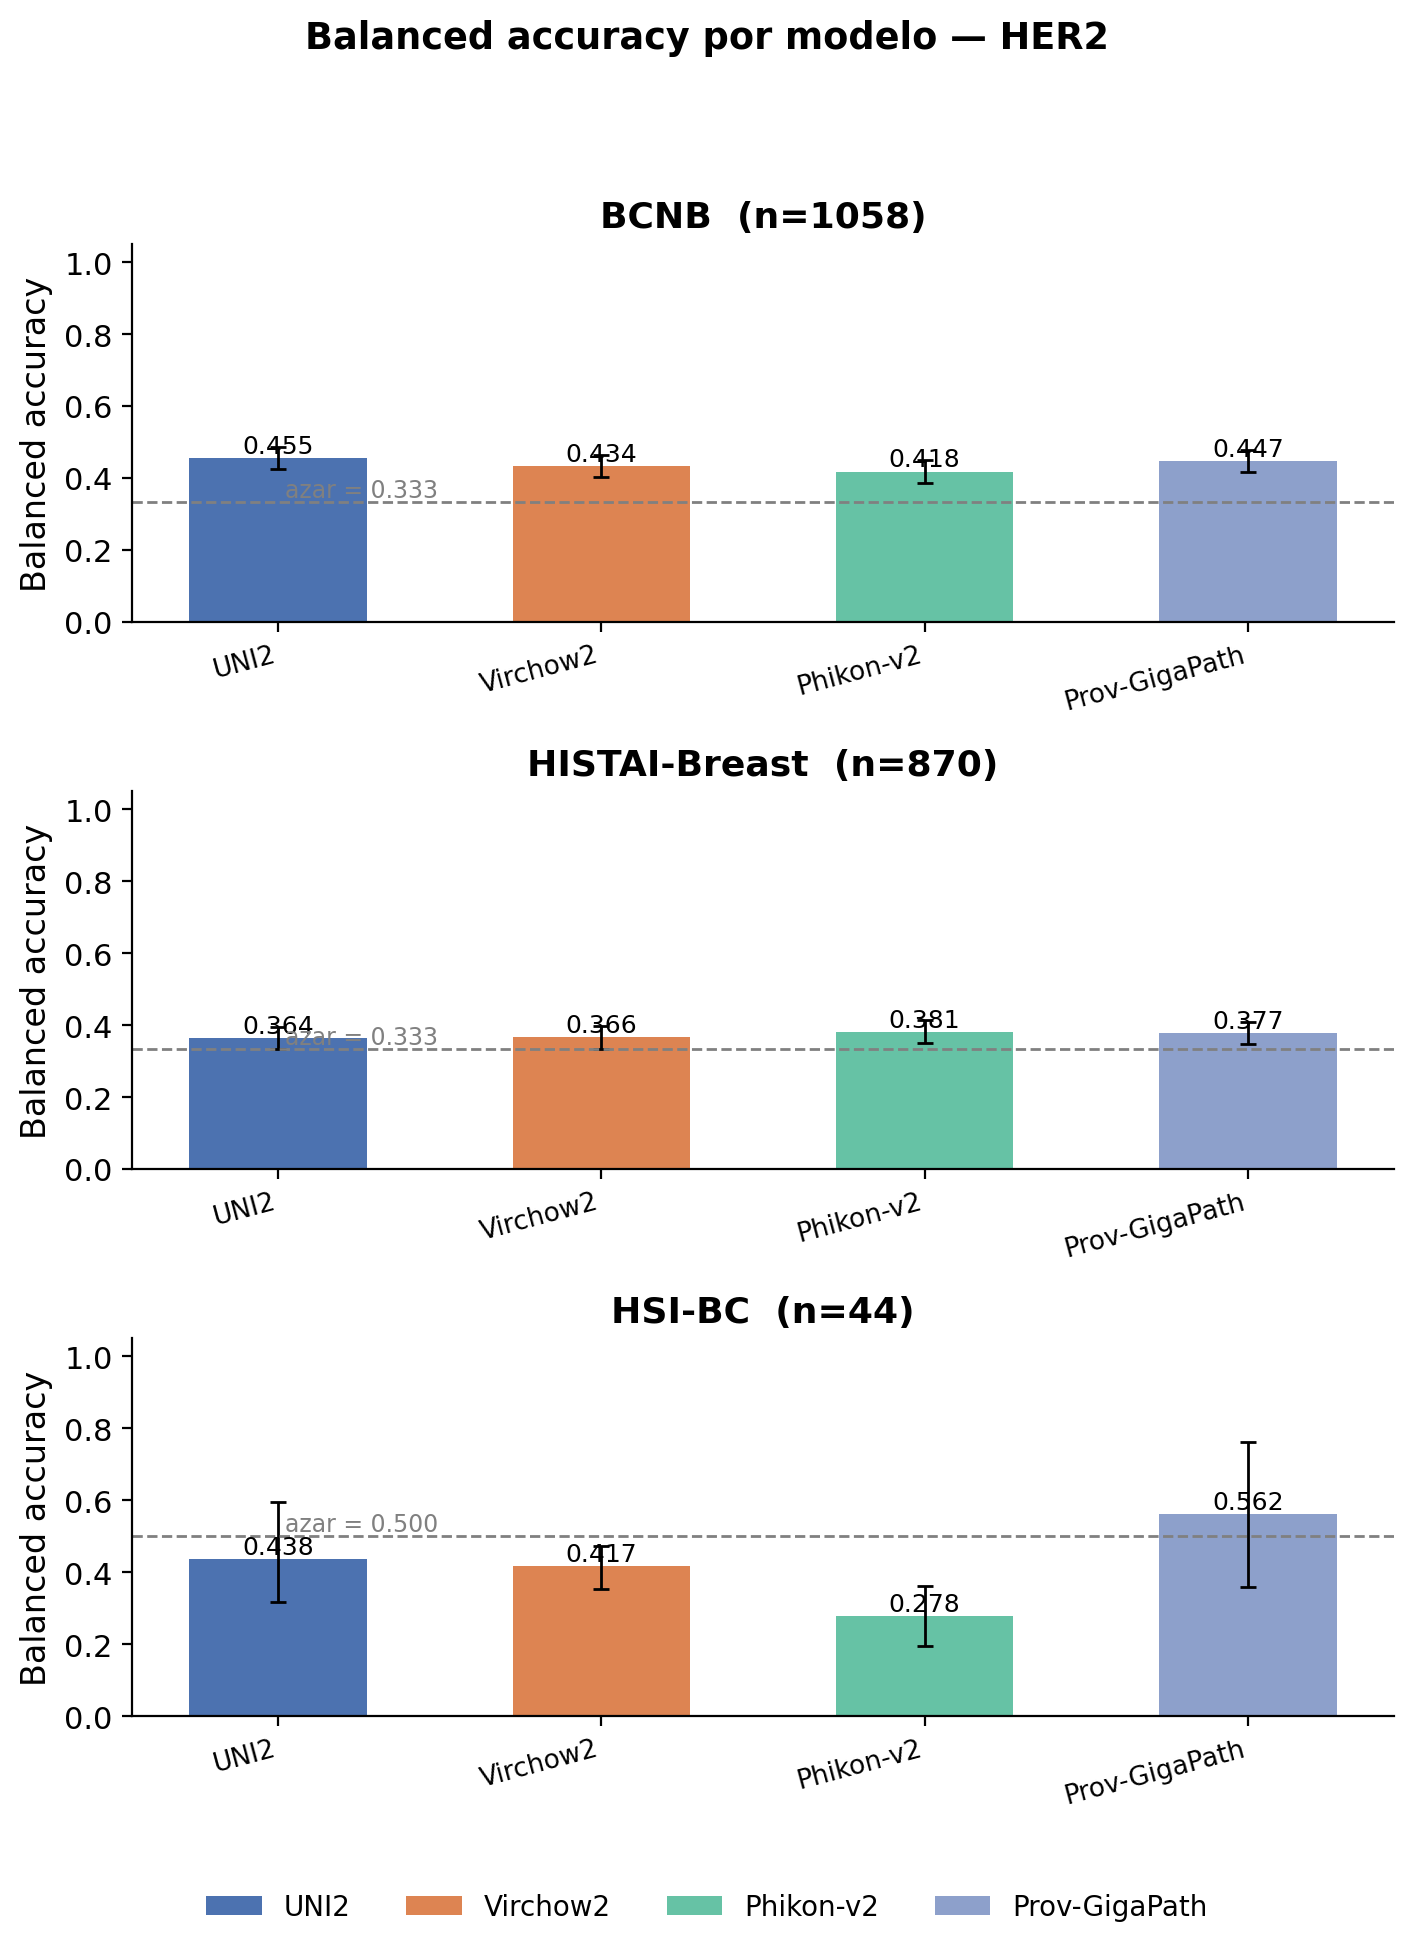
\includegraphics[width=0.75\textwidth]{figures/balanced_accuracy/her2}
\caption{Balanced accuracy por modelo y conjunto de datos en la tarea HER2. Barras de error: IC 95\% bootstrap.}
\label{fig:ba_her2}
\end{figure}

Los valores numéricos completos se presentan en las
Tablas~\ref{tab:anexo_her2_utilidad}; \ref{tab:anexo_her2_sensibilidad}--\ref{tab:anexo_her2_sensibilidad_hsibc};
\ref{tab:anexo_her2_fairness}--\ref{tab:anexo_her2_fairness_hsibc}; y \ref{tab:anexo_her2_crossdataset}
(Apéndice~\ref{anexo:resultados_completos}).

% En síntesis: en las cohortes con tamaño muestral suficiente (BCNB, HISTAI-Breast), no hay evidencia de sesgo sistemático por edad; en HSI-BC las brechas son altas pero el tamaño de la cohorte impide distinguir sesgo real de ruido, por lo que el resultado es no concluyente, no una confirmación de equidad.

\subsubsection{Equidad entre subgrupos}

En BCNB, las brechas de \textit{balanced accuracy} por edad varían según el modelo. UNI2 y Phikon-v2 presentan las brechas más altas, de 0.113 y 0.105, respectivamente; en ambos casos, el grupo de $\geq 70$ años obtiene el mayor desempeño y el grupo de $<50$ años el menor. Virchow2 y Prov-GigaPath presentan brechas menores, de 0.032 y 0.019. En HISTAI-Breast, las brechas oscilan entre 0.022 y 0.065, aunque la dirección de la diferencia no es consistente entre modelos. Por ejemplo, el grupo de mayor desempeño varía según el encoder evaluado.

En HSI-BC, solo los grupos de 50 a 70 años y de $\geq 70$ años cumplen el umbral mínimo de inclusión. Las brechas estimadas varían entre 0.003 y 0.123, pero los intervalos de confianza son amplios debido al reducido tamaño de los subgrupos, de $n=26$ y $n=14$. En consecuencia, los resultados de HSI-BC deben considerarse exploratorios y no permiten inferir de manera robusta la presencia o ausencia de disparidad por edad. El detalle numérico se presenta en las Tablas~\ref{tab:anexo_her2_fairness} a \ref{tab:anexo_her2_fairness_hsibc}.

\subsubsection{Generalización cross-dataset}

La transferencia entre BCNB e HISTAI-Breast presenta caídas de \textit{balanced accuracy} moderadas, aunque asimétricas. Al entrenar en BCNB y evaluar en HISTAI-Breast, las caídas oscilan entre 0.075 y 0.108, equivalentes a 16.5\% a 24.1\%. En la dirección inversa, las caídas se encuentran entre 0.031 y 0.055, equivalentes a 8.4\% a 14.4\%. Este patrón es compatible con una mayor proximidad entre ambas cohortes que la observada respecto de HSI-BC; sin embargo, el diseño no permite atribuir esta diferencia exclusivamente a similitudes morfológicas, ya que pueden intervenir factores de adquisición, composición clínica, prevalencia de clases y calidad de las etiquetas.

La transferencia hacia HSI-BC presenta caídas mayores y debe interpretarse con cautela. Cuando BCNB o HISTAI-Breast actúan como fuente, la \textit{balanced accuracy} OOD disminuye entre 0.179 y 0.447, con valores que alcanzan 0.000 para Prov-GigaPath. Estas comparaciones combinan un cambio de cohorte con un cambio en el número de clases efectivamente evaluadas, ya que HSI-BC no contiene la categoría HER2 2+. Por ello, no son directamente comparables con las transferencias entre BCNB e HISTAI-Breast, donde las tres categorías están presentes.

Cuando HSI-BC actúa como fuente de entrenamiento, algunos modelos presentan valores OOD superiores a sus valores ID. Por ejemplo, Phikon-v2 obtiene un $\Delta_{\text{OOD}}=-0.249$ al evaluar en BCNB. Este resultado no debe interpretarse como generalización superior, sino como una consecuencia posible de la estimación inestable del desempeño ID en una cohorte pequeña y con dos clases. Los resultados completos se presentan en la Tabla~\ref{tab:anexo_her2_crossdataset}.

% ---------------------------------------------------------------------
\begin{figure}[htbp]
\centering
\begin{subfigure}[b]{0.3\textwidth}
\centering
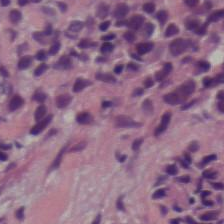
\includegraphics[width=\textwidth]{figures/ejemplos_clase/parches/her2_01plus}
\caption{0/1+}
\end{subfigure}\hfill
\begin{subfigure}[b]{0.3\textwidth}
\centering
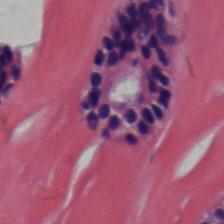
\includegraphics[width=\textwidth]{figures/ejemplos_clase/parches/her2_2plus}
\caption{2+}
\end{subfigure}\hfill
\begin{subfigure}[b]{0.3\textwidth}
\centering
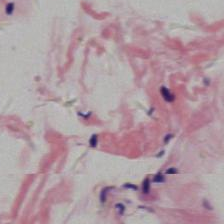
\includegraphics[width=\textwidth]{figures/ejemplos_clase/parches/her2_3plus}
\caption{3+}
\end{subfigure}
\caption{Ejemplos representativos de parches para cada clase de HER2.}
\label{fig:ejemplos_her2}
\end{figure}

En conjunto, T1-HER2 muestra una utilidad predictiva limitada bajo el protocolo de extracción de características congeladas y clasificación a nivel de paciente utilizado en este estudio. Incluso en las cohortes de mayor tamaño, la \textit{balanced accuracy} supera el nivel de referencia por un margen acotado y la sensibilidad se concentra en la categoría 2+. Este comportamiento es compatible con la relación indirecta entre la morfología H\&E y un biomarcador definido mediante inmunohistoquímica, así como con el efecto del desbalance de clases. No obstante, el diseño no permite separar la contribución de estos factores.

Las diferencias entre cohortes son coherentes con las limitaciones documentadas en el Capítulo~\ref{cap:caracterizacion_datasets}. BCNB presenta el desempeño más alto y estable; HISTAI-Breast alcanza resultados menores, en un contexto donde la obtención de biomarcadores desde texto libre puede introducir incertidumbre de etiquetado; y HSI-BC concentra la mayor inestabilidad debido a su tamaño reducido y su limitada representación de clases. Estas asociaciones respaldan la necesidad de interpretar la utilidad y la equidad en función de la calidad, trazabilidad y tamaño de cada cohorte, más que como propiedades exclusivas del modelo fundacional.

Respecto de la equidad por edad, los resultados no muestran una dirección de favorecimiento que sea consistente entre modelos y cohortes. En BCNB e HISTAI-Breast se observan brechas de magnitud variable, mientras que HSI-BC no posee potencia estadística suficiente para establecer conclusiones robustas. Por tanto, los resultados deben interpretarse como una caracterización exploratoria de posibles disparidades, no como evidencia definitiva de equidad o inequidad por edad.

% ---------------------------------------------------------------------
\subsection{T2: Subtipo molecular}
\label{sec:resultado_molsub}

\subsubsection{Descripción de la tarea y distribución de clases}

La tarea T2-MOLSUB consiste en clasificar el subtipo molecular del cáncer de mama en cuatro categorías: Luminal A, Luminal B, HER2+ y Triple Negativo. En BCNB ($n=1058$) la distribución es relativamente equilibrada (Luminal B 35.2\,\%, Luminal A 27.2\,\%, HER2+ 25.8\,\%, Triple Negativo 11.8\,\%); en HISTAI-Breast ($n=842$) domina Luminal B (41.6\,\%) y Triple Negativo es minoritaria (8.8\,\%); en HSI-BC ($n=44$) Luminal B concentra el 63.6\,\% de los casos y HER2+ cuenta con solo 3 casos. La Figura~\ref{fig:dist_molsub} muestra la distribución de clases por conjunto de datos y la Figura~\ref{fig:ejemplos_molsub} ejemplos representativos por clase.

\begin{figure}[htbp]
\centering
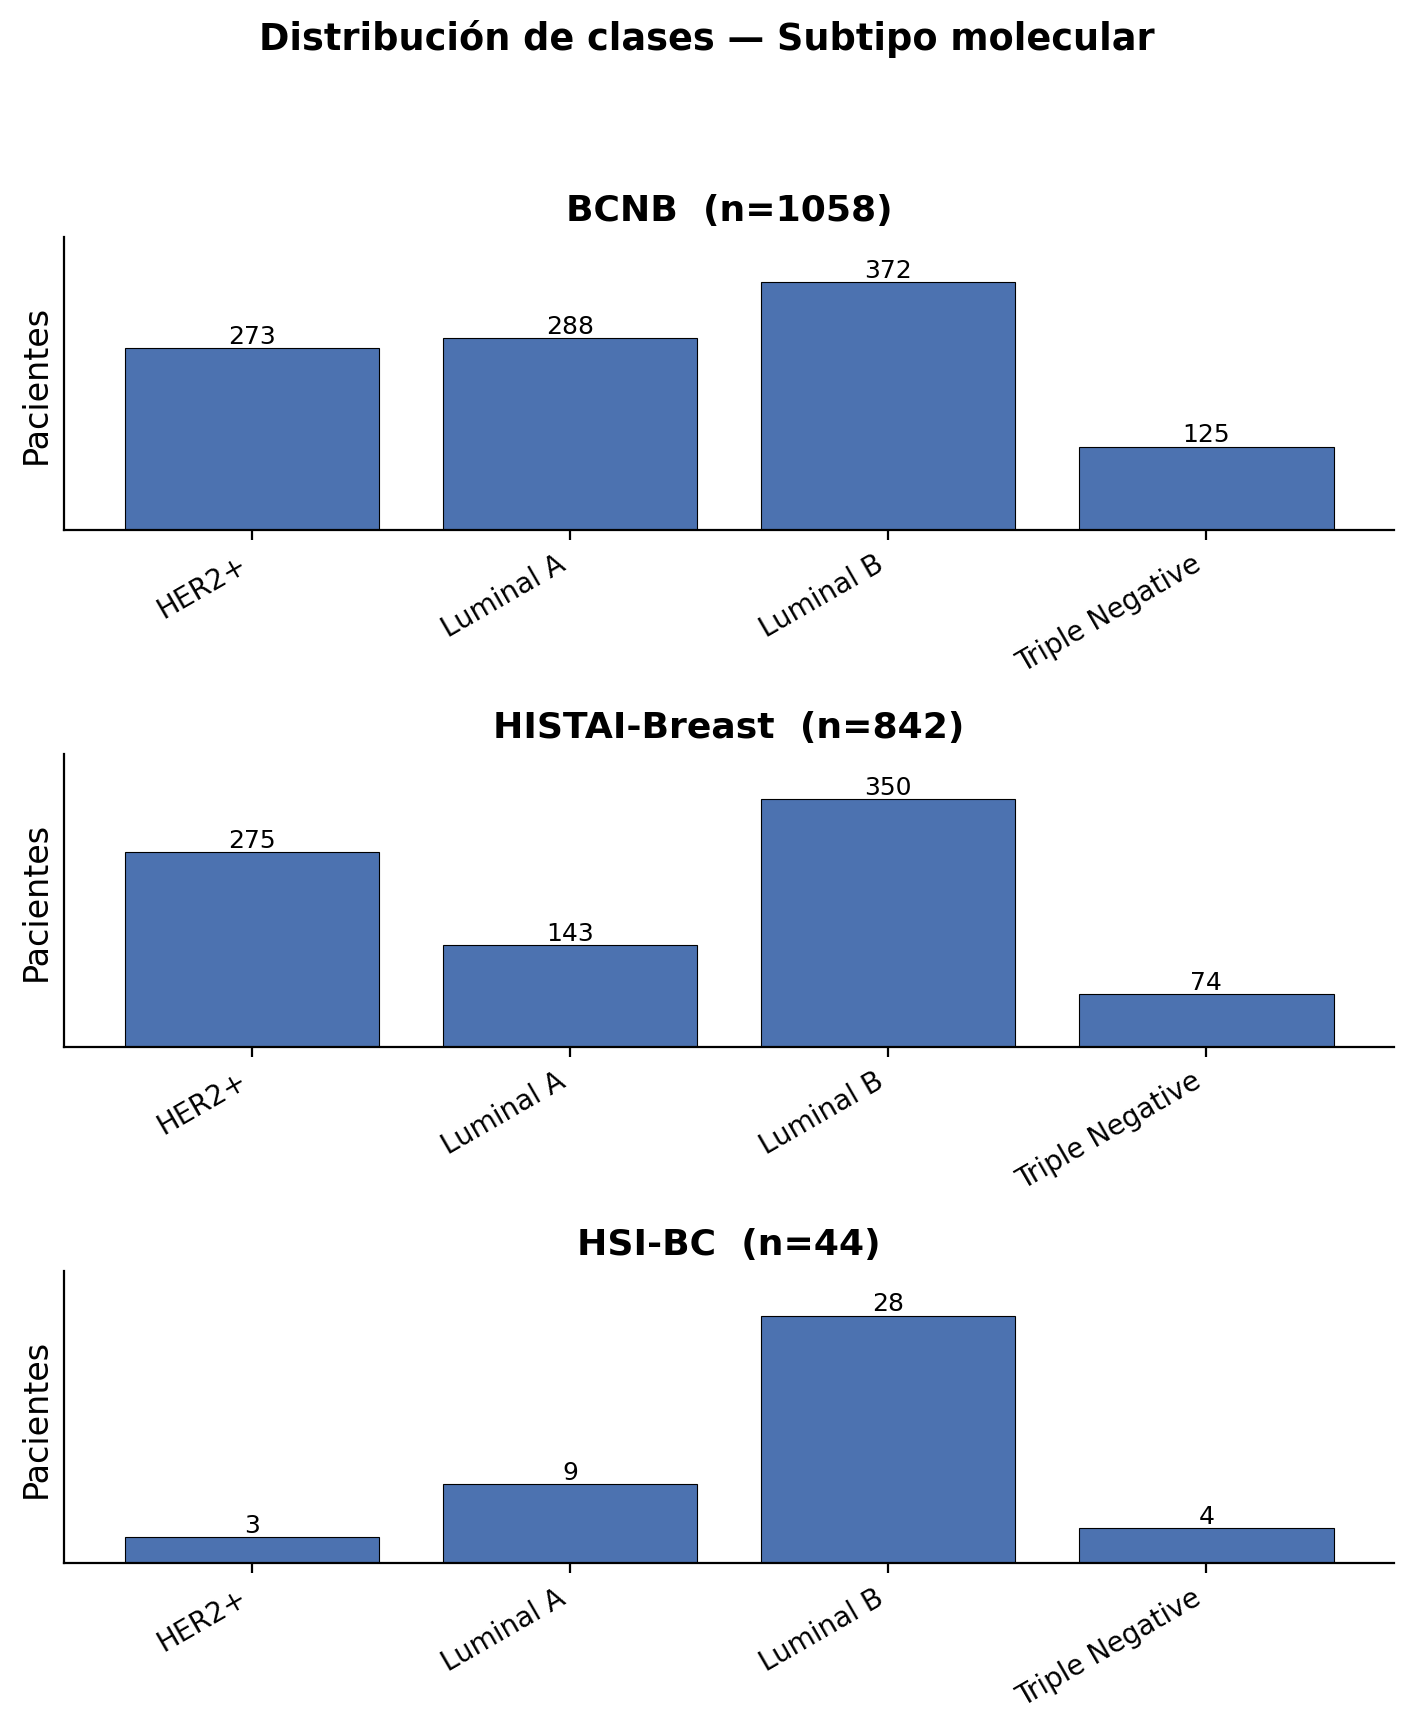
\includegraphics[width=0.72\textwidth]{figures/distribucion_clases/molsub}
\caption{Distribución de clases de la tarea MolSub por conjunto de datos.}
\label{fig:dist_molsub}
\end{figure}

\begin{figure}[htbp]
\centering
\begin{subfigure}[b]{0.45\textwidth}
\centering
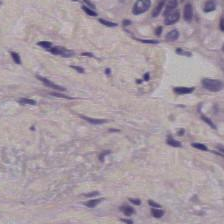
\includegraphics[width=\textwidth]{figures/ejemplos_clase/parches/molsub_her2plus}
\caption{HER2+}
\end{subfigure}\hfill
\begin{subfigure}[b]{0.45\textwidth}
\centering
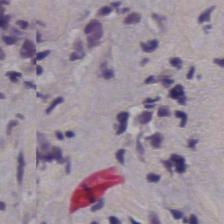
\includegraphics[width=\textwidth]{figures/ejemplos_clase/parches/molsub_luminal_a}
\caption{Luminal A}
\end{subfigure}
\\[2ex]
\begin{subfigure}[b]{0.45\textwidth}
\centering
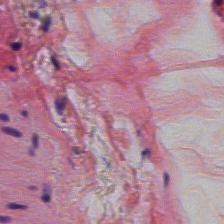
\includegraphics[width=\textwidth]{figures/ejemplos_clase/parches/molsub_luminal_b}
\caption{Luminal B}
\end{subfigure}\hfill
\begin{subfigure}[b]{0.45\textwidth}
\centering
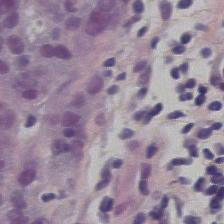
\includegraphics[width=\textwidth]{figures/ejemplos_clase/parches/molsub_triple_neg}
\caption{Triple Negative}
\end{subfigure}
\caption{Ejemplos representativos de parches para cada clase de MolSub.}
\label{fig:ejemplos_molsub}
\end{figure}

La Figura~\ref{fig:ejemplos_her2} presenta ejemplos representativos de parches asociados a cada categoría. Estas imágenes ilustran la variabilidad visual de las muestras.

\subsubsection{Desempeño por modelo y dataset}

En BCNB, UNI2 alcanza la mayor \textit{balanced accuracy}, de 0.482 con IC 95\% de [0.450, 0.514], seguido de Prov-GigaPath con 0.472. Virchow2 y Phikon-v2 obtienen valores de 0.427 y 0.434, respectivamente. El AUC macro varía entre 0.697 y 0.740, valores superiores a los observados en la tarea T1-HER2 sobre la misma cohorte. Bajo el protocolo utilizado, este resultado indica una mayor capacidad discriminativa para T2-MOLSUB que para T1-HER2; sin embargo, esta diferencia también puede estar influida por la definición de las etiquetas, su distribución y su calidad.

En HISTAI-Breast, la \textit{balanced accuracy} disminuye al intervalo de 0.327 a 0.361. En HSI-BC, donde el nivel de referencia para cuatro clases es 0.25, UNI2 y Prov-GigaPath alcanzan 0.317 y 0.334, respectivamente, mientras que Virchow2 y Phikon-v2 quedan por debajo de este valor. Dado que HSI-BC contiene solo 44 pacientes y presenta categorías con escasa representación, estas diferencias deben interpretarse como estimaciones inestables y no como un ordenamiento concluyente entre modelos.

El análisis por clase evidencia una heterogeneidad relevante. Luminal B es la categoría con mayor sensibilidad en BCNB y en HISTAI-Breast, con valores entre 0.492 y 0.617. HER2+ presenta sensibilidades entre 0.262 y 0.403 en las cohortes grandes. Triple Negativo alcanza sensibilidades de 0.448 a 0.568 en BCNB, pero disminuye a 0.216 a 0.230 en HISTAI-Breast. En HSI-BC, ningún modelo identifica los tres casos de HER2+, por lo que esa sensibilidad igual a cero debe interpretarse principalmente en función del tamaño extremadamente reducido de la categoría.

\begin{figure}[htbp]
\centering
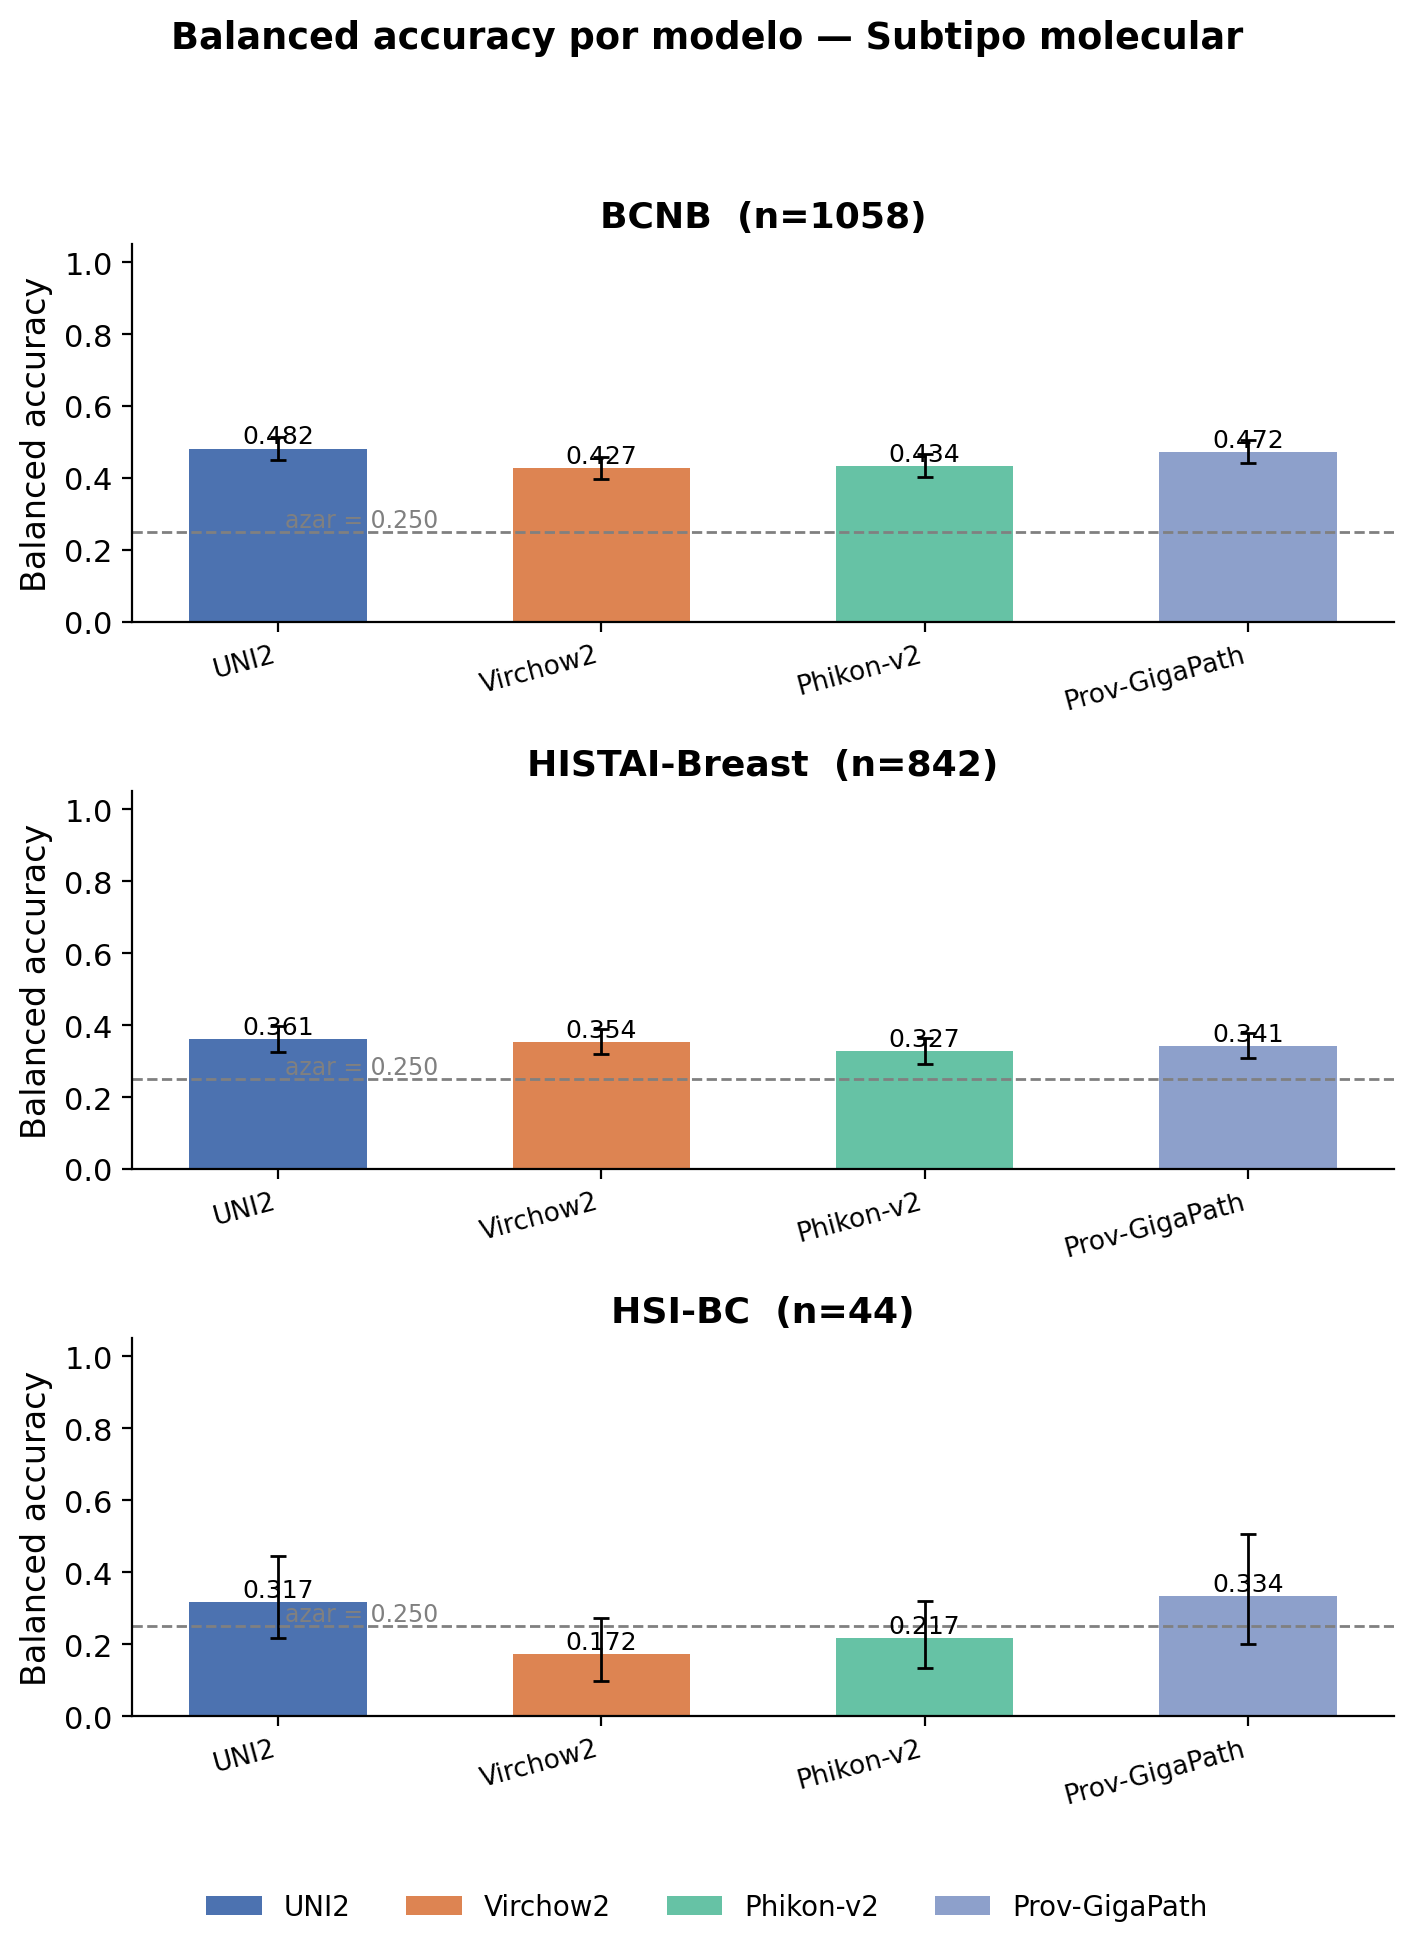
\includegraphics[width=0.72\textwidth]{figures/balanced_accuracy/molsub}
\caption{Balanced accuracy por modelo y conjunto de datos en la tarea MolSub. Barras de error: IC 95\% bootstrap.}
\label{fig:ba_molsub}
\end{figure}

Los valores numéricos completos se presentan en las
Tablas~\ref{tab:anexo_molsub_utilidad}; \ref{tab:anexo_molsub_sensibilidad}--\ref{tab:anexo_molsub_sensibilidad_hsibc};
\ref{tab:anexo_molsub_fairness}--\ref{tab:anexo_molsub_fairness_hsibc}; y \ref{tab:anexo_molsub_crossdataset}
(Apéndice~\ref{anexo:resultados_completos}).

\subsubsection{Equidad entre subgrupos}

En BCNB, las brechas de \textit{balanced accuracy} por edad varían entre modelos. Virchow2 y Phikon-v2 presentan las brechas más bajas, de 0.010 y 0.023, respectivamente, mientras que UNI2 y Prov-GigaPath alcanzan brechas de 0.078 y 0.041. La dirección de las diferencias no es uniforme: el grupo de menor edad obtiene el mayor desempeño en UNI2 y Phikon-v2, mientras que el grupo de $\geq 70$ años registra el menor desempeño en UNI2 y Prov-GigaPath. Por tanto, no se observa un grupo etario favorecido de manera consistente entre los cuatro modelos.

En HISTAI-Breast, las brechas varían entre 0.063 para UNI2 y 0.107 para Virchow2. Los grupos con mejor desempeño también cambian según el modelo: el grupo de $<50$ años obtiene la mayor \textit{balanced accuracy} en UNI2 y Phikon-v2, mientras que el grupo de $\geq 70$ años lo hace en Virchow2 y Prov-GigaPath. Estas diferencias deben interpretarse considerando que la cohorte analítica de HISTAI-Breast presenta un sesgo de selección hacia pacientes de mayor edad, debido al filtrado por disponibilidad de biomarcadores.

En HSI-BC, solo los grupos de 50 a 70 años y de $\geq 70$ años cumplen el criterio mínimo de inclusión. Las brechas estimadas varían entre 0.074 y 0.426. La mayor corresponde a Prov-GigaPath, con una \textit{balanced accuracy} de 0.593 en el grupo de 50 a 70 años y de 0.190 en el grupo de $\geq 70$ años. Sin embargo, estas estimaciones se basan en subgrupos de $n=26$ y $n=14$, respectivamente, y sus intervalos de confianza son amplios. En consecuencia, este resultado debe considerarse exploratorio y no permite establecer una disparidad por edad de manera concluyente.

Además, en cohortes pequeñas y tareas multiclase, la comparación de \textit{balanced accuracy} por subgrupo puede estar condicionada por la ausencia o escasa presencia de algunas categorías dentro de cada grupo etario. Por esta razón, las brechas reportadas describen diferencias observadas en esta muestra, pero no deben interpretarse como estimaciones estables de equidad poblacional.

\subsubsection{Generalización cross-dataset}

La transferencia desde BCNB hacia HISTAI-Breast presenta caídas de \textit{balanced accuracy} entre 0.070 y 0.163, equivalentes a pérdidas relativas de 16.5\% a 34.6\%. La magnitud de la caída varía entre modelos: Virchow2 presenta la menor reducción, mientras que Prov-GigaPath y UNI2 registran las mayores. Estos resultados indican una pérdida de rendimiento al trasladar el clasificador a una cohorte externa, aunque el diseño no permite separar la contribución de las diferencias de adquisición, composición clínica, prevalencia de subtipos y calidad de las etiquetas.

La transferencia hacia HSI-BC presenta resultados más variables. UNI2 y Virchow2 registran caídas de 0.253 y 0.205, respectivamente; Phikon-v2 disminuye 0.108; y Prov-GigaPath presenta una diferencia reducida, de 0.004. Este último resultado no debe interpretarse por sí solo como evidencia de robustez superior, ya que HSI-BC es una cohorte pequeña, con distribución de clases distinta y categorías muy escasas. Las diferencias de rendimiento OOD hacia esta cohorte dependen, además, de la limitada precisión de las estimaciones ID y OOD.

Cuando HSI-BC se utiliza como conjunto de entrenamiento, algunos modelos presentan valores OOD superiores a su desempeño ID. Por ejemplo, Virchow2 presenta un $\Delta_{\text{OOD}}=-0.096$ al evaluar en BCNB. Al igual que en T1-HER2, este patrón es compatible con la inestabilidad de la estimación ID en una cohorte pequeña y no debe interpretarse como evidencia de mejor generalización externa. Los resultados completos se presentan en la Tabla~\ref{tab:anexo_molsub_crossdataset}.

% final

En conjunto, T2-MOLSUB presenta una utilidad predictiva mayor que T1-HER2 en BCNB, particularmente al considerar el AUC macro. Bajo este protocolo, las representaciones fundacionales contienen información más útil para discriminar subtipos moleculares que para clasificar el estado HER2 aislado. Sin embargo, este resultado no permite concluir que la diferencia provenga exclusivamente de una señal morfológica más fuerte, dado que las tareas también difieren en definición de etiquetas, distribución de clases y posibles fuentes de incertidumbre en los metadatos clínicos.

El desempeño disminuye de forma consistente desde BCNB hacia HISTAI-Breast y, con mayor inestabilidad, hacia HSI-BC. Este gradiente es compatible con las limitaciones documentadas en la caracterización de las cohortes: BCNB presenta una mayor estabilidad de resultados; HISTAI-Breast incorpora incertidumbre asociada a la extracción de biomarcadores desde texto libre; y HSI-BC combina tamaño muestral reducido con categorías poco representadas. Estas condiciones afectan simultáneamente la utilidad predictiva, la precisión de las estimaciones de equidad y la interpretación de la generalización externa.

Respecto de la equidad por edad, no se observa un patrón de favorecimiento consistente entre modelos ni entre cohortes. Las brechas de BCNB e HISTAI-Breast describen diferencias de magnitud variable, mientras que la brecha elevada de Prov-GigaPath en HSI-BC requiere validación en una cohorte mayor. Por tanto, los resultados caracterizan posibles disparidades bajo las condiciones evaluadas, pero no permiten afirmar de manera definitiva ni la presencia ni la ausencia de inequidad por edad.


% ---------------------------------------------------------------------
\subsection{T3: Sitio anatómico}
\label{sec:resultado_site}

\subsubsection{Descripción de la tarea y distribución de clases}

La tarea T3-SITE clasifica el sitio anatómico del tumor colorrectal en nueve categorías: colon derecho, colon transverso, colon izquierdo, sigmoide, rectosigmoide, recto, colon sin especificar, otro y metástasis hepática. En HISTAI-CRC-B1 ($n=878$) predominan sigmoide (24.0\,\%), recto (18.2\,\%) y colon derecho (15.4\,\%); en SurGen ($n=765$) dominan recto (29.8\,\%) y colon derecho (22.9\,\%); en HISTAI-CRC-B2 ($n=57$) la clase metástasis hepática está ausente y varias clases cuentan con menos de 5 casos (colon izquierdo 2, rectosigmoide 1, transverso 1). La Figura~\ref{fig:dist_site} muestra la distribución de clases por conjunto de datos y la Figura~\ref{fig:ejemplos_site} ejemplos representativos por clase.

\begin{figure}[htbp]
\centering
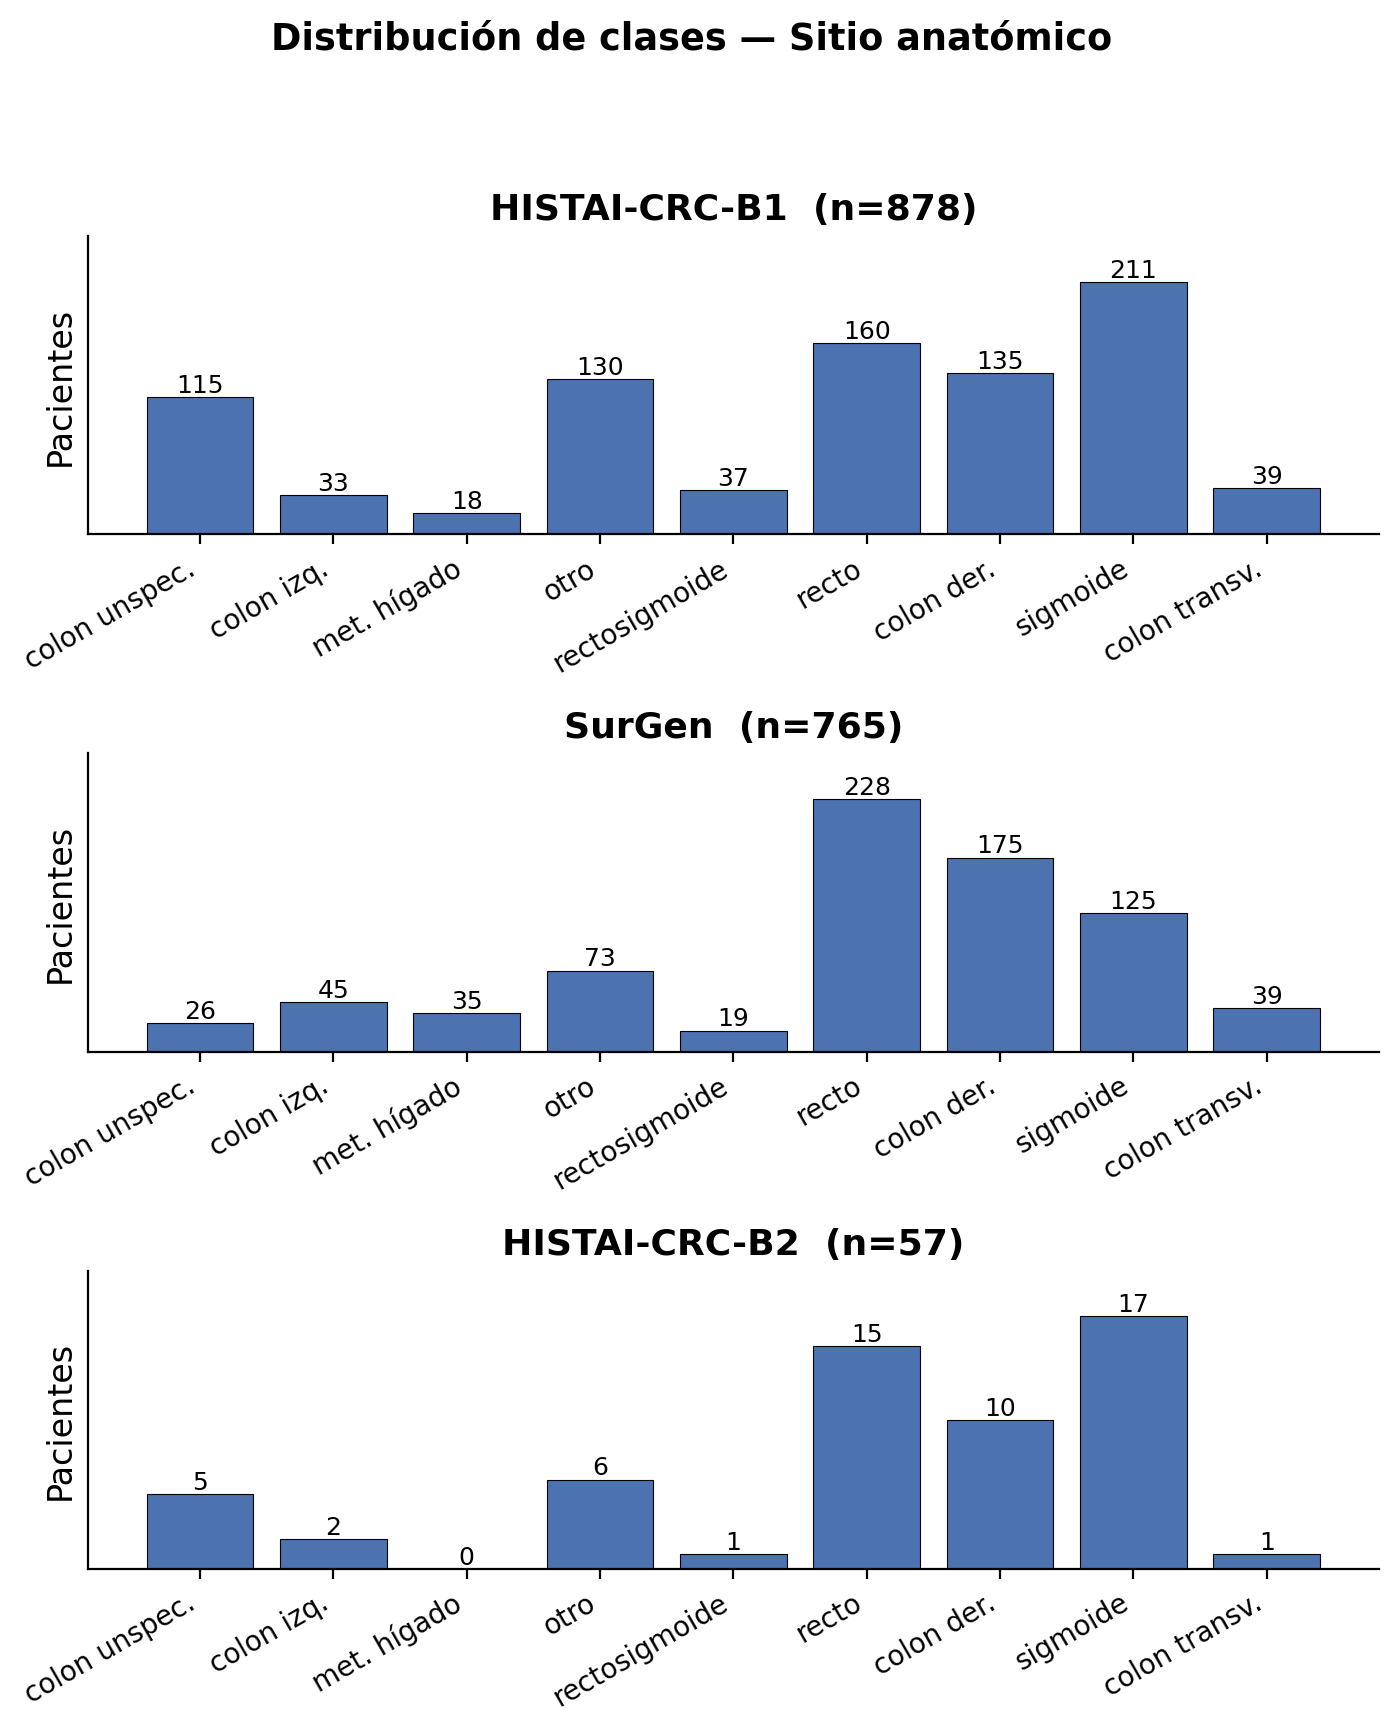
\includegraphics[width=0.72\textwidth]{figures/distribucion_clases/site}
\caption{Distribución de clases de la tarea Site por conjunto de datos.}
\label{fig:dist_site}
\end{figure}

\begin{figure}[htbp]
\centering
\begin{subfigure}[b]{0.3\textwidth}
\centering
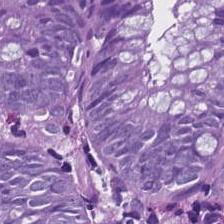
\includegraphics[width=\textwidth]{figures/ejemplos_clase/parches/site_colon_sin_especificar}
\caption{Colon sin especificar}
\end{subfigure}\hfill
\begin{subfigure}[b]{0.3\textwidth}
\centering
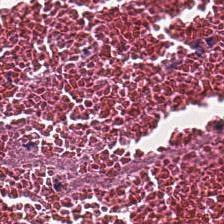
\includegraphics[width=\textwidth]{figures/ejemplos_clase/parches/site_colon_izquierdo}
\caption{Colon izquierdo}
\end{subfigure}\hfill
\begin{subfigure}[b]{0.3\textwidth}
\centering
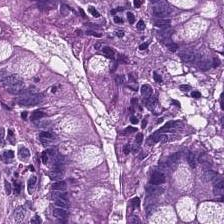
\includegraphics[width=\textwidth]{figures/ejemplos_clase/parches/site_met_higado}
\caption{Metástasis hepática}
\end{subfigure}
\\[2ex]
\begin{subfigure}[b]{0.3\textwidth}
\centering
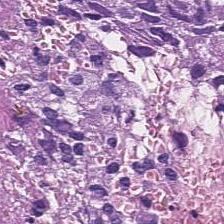
\includegraphics[width=\textwidth]{figures/ejemplos_clase/parches/site_otro}
\caption{Otro}
\end{subfigure}\hfill
\begin{subfigure}[b]{0.3\textwidth}
\centering
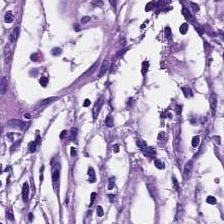
\includegraphics[width=\textwidth]{figures/ejemplos_clase/parches/site_rectosigmoide}
\caption{Rectosigmoide}
\end{subfigure}\hfill
\begin{subfigure}[b]{0.3\textwidth}
\centering
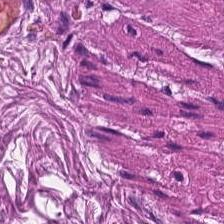
\includegraphics[width=\textwidth]{figures/ejemplos_clase/parches/site_recto}
\caption{Recto}
\end{subfigure}
\\[2ex]
\begin{subfigure}[b]{0.3\textwidth}
\centering
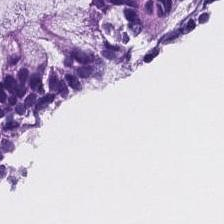
\includegraphics[width=\textwidth]{figures/ejemplos_clase/parches/site_colon_derecho}
\caption{Colon derecho}
\end{subfigure}\hfill
\begin{subfigure}[b]{0.3\textwidth}
\centering
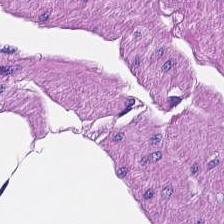
\includegraphics[width=\textwidth]{figures/ejemplos_clase/parches/site_sigmoide}
\caption{Sigmoide}
\end{subfigure}\hfill
\begin{subfigure}[b]{0.3\textwidth}
\centering
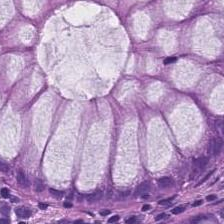
\includegraphics[width=\textwidth]{figures/ejemplos_clase/parches/site_colon_transverso}
\caption{Colon transverso}
\end{subfigure}
\caption{Ejemplos representativos de parches para cada clase de Site.}
\label{fig:ejemplos_site}
\end{figure}

La Figura~\ref{fig:ejemplos_site} presenta ejemplos representativos de parches para las categorías anatómicas evaluadas. Estos ejemplos permiten ilustrar la diversidad visual de las muestras.

\subsubsection{Desempeño por modelo y dataset}

En la tarea T3-SITE, el nivel de referencia de la \textit{balanced accuracy} depende del número de clases presentes en cada cohorte. HISTAI-CRC-B1 y SurGen contienen nueve categorías, por lo que el nivel de referencia uniforme corresponde aproximadamente a 0.111. HISTAI-CRC-B2 contiene ocho categorías, ya que metástasis hepática está ausente, por lo que su nivel de referencia corresponde a 0.125.

SurGen presenta el mayor desempeño absoluto, con valores de \textit{balanced accuracy} entre 0.309 y 0.367; UNI2 alcanza 0.367 con IC 95\% de [0.331, 0.403]. En HISTAI-CRC-B1, los cuatro modelos obtienen valores entre 0.203 y 0.210. Aunque este desempeño es inferior al de SurGen, se encuentra por sobre el nivel de referencia de una tarea con nueve clases. En HISTAI-CRC-B2, los valores varían entre 0.094 y 0.138, cercanos al nivel de referencia correspondiente a ocho clases y acompañados de intervalos de confianza amplios. Por tanto, esta cohorte no permite una estimación precisa de la utilidad predictiva de los modelos para esta tarea.

La sensibilidad por clase es heterogénea entre cohortes. En SurGen, recto, colon derecho y metástasis hepática alcanzan sensibilidades relativamente altas, con valores máximos de 0.684, 0.480 y 0.886, respectivamente. En HISTAI-CRC-B1, colon derecho y sigmoide alcanzan sensibilidades entre 0.384 y 0.459, mientras que metástasis hepática no es identificada por ninguno de los modelos, a pesar de estar presente en 18 pacientes. Las categorías rectosigmoide y colon transverso muestran sensibilidades bajas en las cohortes evaluadas, lo que coincide con su baja representación.

El contraste entre la sensibilidad de metástasis hepática en SurGen y en HISTAI-CRC-B1 es compatible con una influencia de la frecuencia de la clase y de su representatividad dentro de cada cohorte. Sin embargo, las cohortes también difieren en adquisición, composición clínica y posibles criterios de anotación, por lo que no es posible atribuir esta diferencia exclusivamente al número de ejemplos disponibles.

\begin{figure}[htbp]
\centering
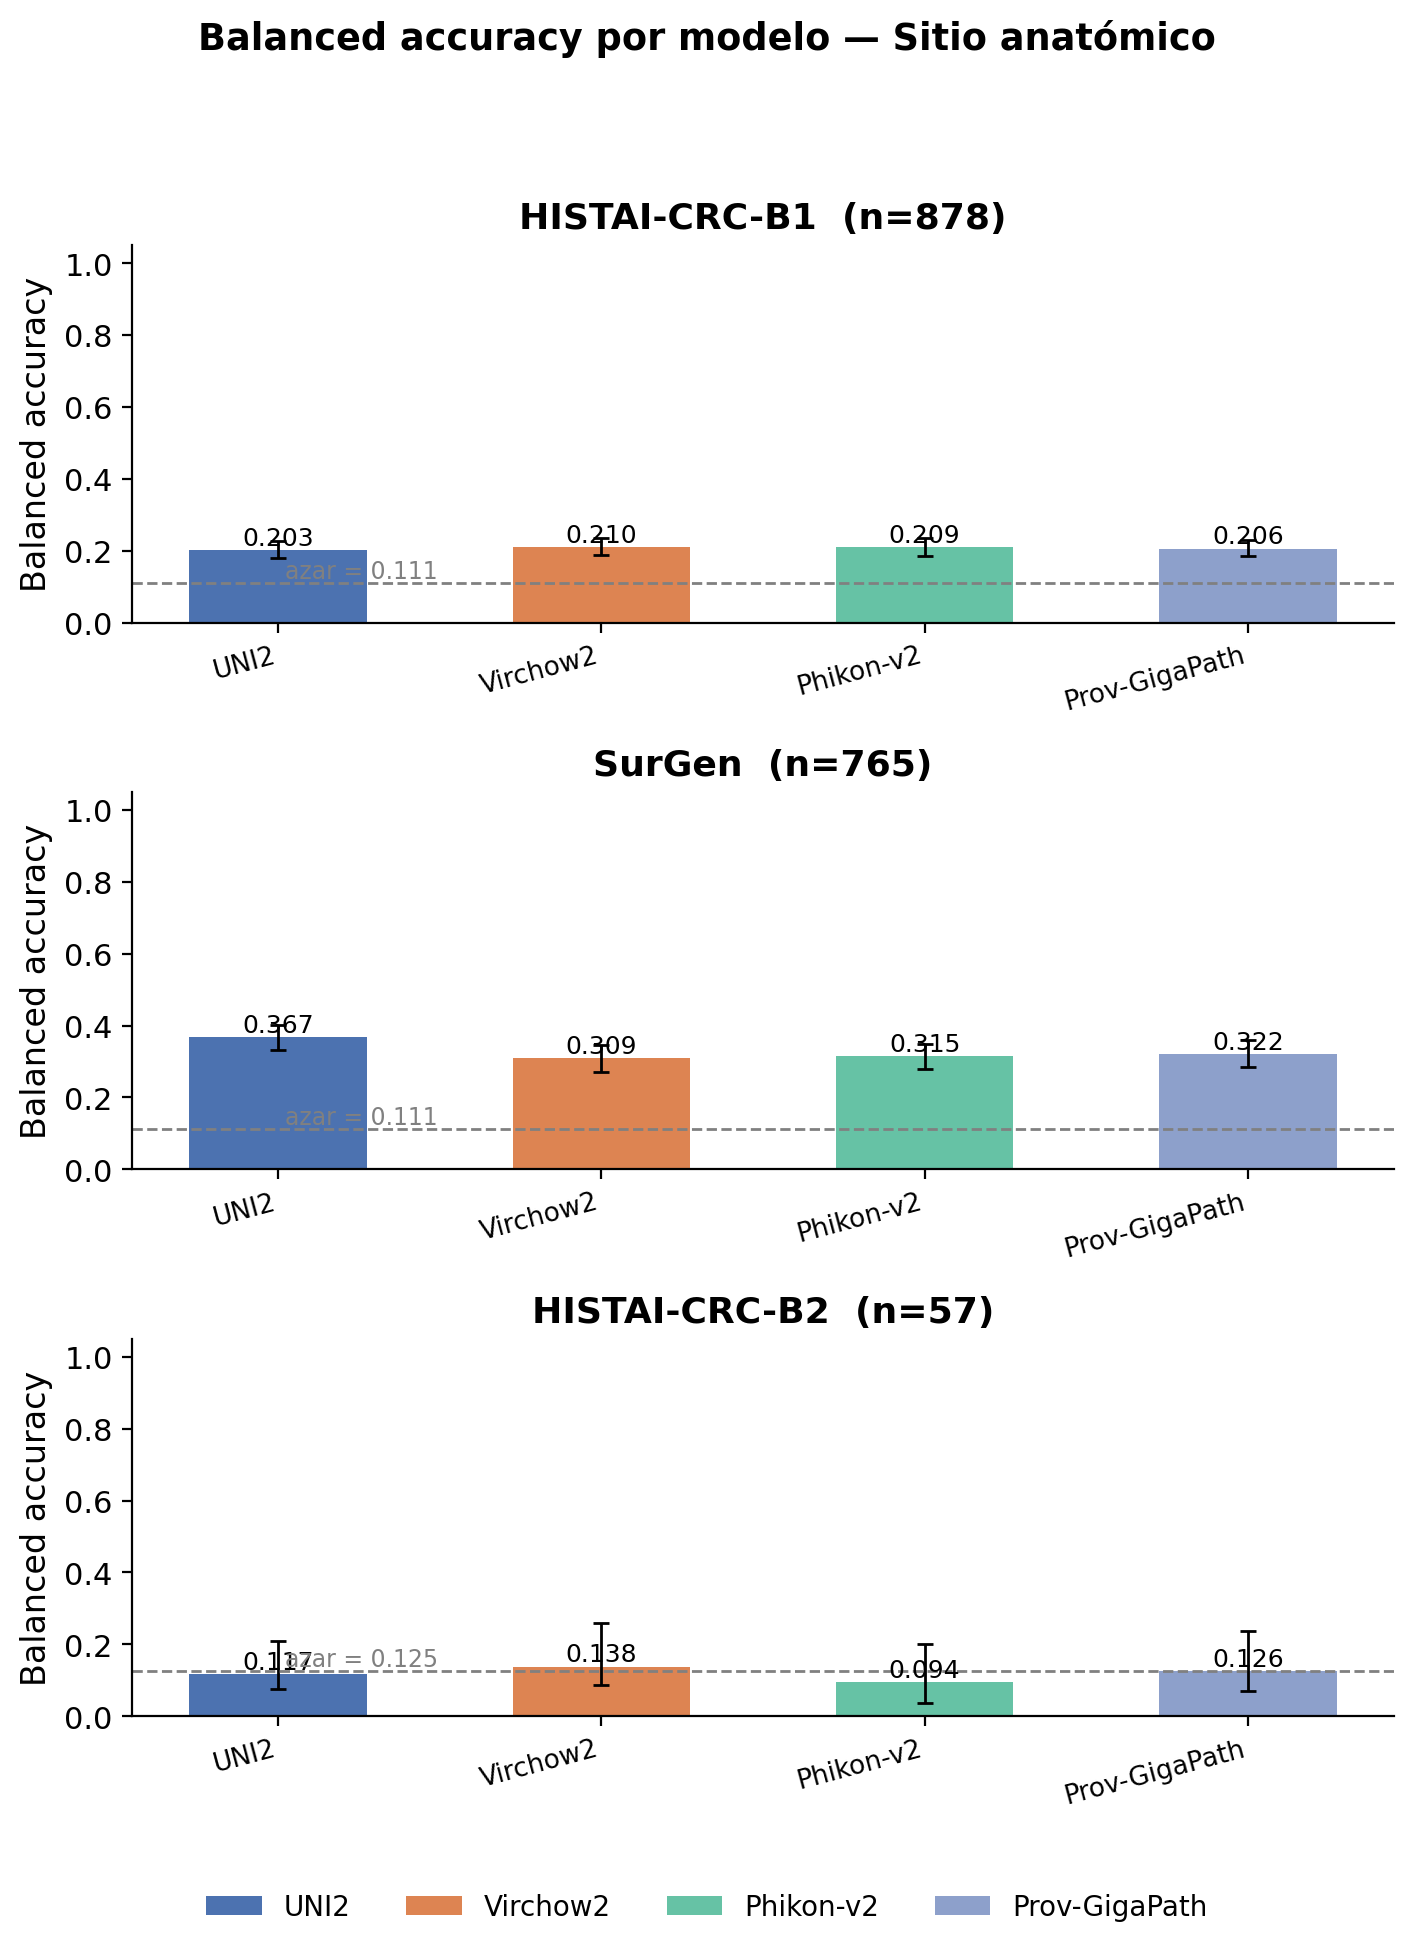
\includegraphics[width=0.72\textwidth]{figures/balanced_accuracy/site}
\caption{Balanced accuracy por modelo y conjunto de datos en la tarea Site. Barras de error: IC 95\% bootstrap.}
\label{fig:ba_site}
\end{figure}

Los valores numéricos completos se presentan en las
Tablas~\ref{tab:anexo_site_utilidad}; \ref{tab:anexo_site_sensibilidad}--\ref{tab:anexo_site_sensibilidad_surgen};
\ref{tab:anexo_site_fairness_edad}--\ref{tab:anexo_site_fairness_edad_surgen};
\ref{tab:anexo_site_fairness_sexo}--\ref{tab:anexo_site_fairness_sexo_surgen}; y
\ref{tab:anexo_site_crossdataset} (Apéndice~\ref{anexo:resultados_completos}).

\subsubsection{Equidad entre subgrupos}

En HISTAI-CRC-B1 y SurGen, las brechas por edad son de magnitud reducida a moderada. En HISTAI-CRC-B1, estas varían entre 0.018 y 0.049; en SurGen, entre 0.026 y 0.072. Las brechas por sexo también son acotadas en estas cohortes, con valores entre 0.026 y 0.046 en HISTAI-CRC-B1 y entre 0.002 y 0.063 en SurGen. No obstante, la dirección de las diferencias varía entre modelos, por lo que no se observa un subgrupo de edad o sexo favorecido de manera consistente.

En HISTAI-CRC-B2, los análisis por edad incluyen únicamente los grupos de 50 a 70 años y de $\geq 70$ años, con $n=25$ y $n=27$, respectivamente. Las brechas estimadas por edad varían entre 0.053 y 0.360. La mayor corresponde a Phikon-v2, cuyo IC 95\% para la brecha es [0.015, 0.778]. Por sexo, los tamaños son de $n=32$ para mujeres y $n=25$ para hombres; Phikon-v2 presenta una diferencia de 0.201, con \textit{balanced accuracy} igual a 0.201 en mujeres y 0.000 en hombres.

Estas estimaciones para HISTAI-CRC-B2 deben interpretarse de forma exploratoria. El tamaño total de la cohorte es reducido, algunas categorías tienen muy pocos pacientes y la composición de clases puede diferir entre subgrupos. En consecuencia, las diferencias observadas no permiten establecer de manera robusta si existe una disparidad real por edad o sexo, ni permiten descartar que parte de ellas sea consecuencia de la variabilidad muestral.

\subsubsection{Generalización cross-dataset}

La generalización cross-dataset muestra caídas relevantes al transferir los clasificadores entre cohortes colorrectales. Cuando SurGen actúa como conjunto de entrenamiento, la transferencia hacia HISTAI-CRC-B1 reduce la \textit{balanced accuracy} entre 0.166 y 0.238, equivalentes a pérdidas relativas de 51.6\% a 64.9\%. La transferencia desde SurGen hacia HISTAI-CRC-B2 también presenta caídas, entre 0.107 y 0.195; sin embargo, estas deben interpretarse con especial cautela debido al tamaño reducido de la cohorte de destino y a la ausencia de una de las categorías anatómicas.

En la dirección HISTAI-CRC-B1 hacia SurGen, las caídas se sitúan entre 0.081 y 0.106, equivalentes a 38.8\% a 50.3\%. La asimetría entre direcciones muestra que la transferibilidad depende tanto de la cohorte de entrenamiento como de la cohorte de evaluación. Este resultado es compatible con diferencias de distribución entre datasets, pero el diseño no permite identificar si estas diferencias provienen principalmente de factores técnicos, composición clínica, distribución de sitios anatómicos o procedimientos de anotación.

Cuando HISTAI-CRC-B2 se utiliza como fuente de entrenamiento, algunos resultados OOD superan el desempeño ID. Dado que el desempeño ID de esta cohorte es cercano al nivel de referencia y se estima sobre solo 57 pacientes, los deltas negativos deben interpretarse como evidencia de inestabilidad de la estimación ID, no como una demostración de generalización externa. Los resultados completos se presentan en la Tabla~\ref{tab:anexo_site_crossdataset}.

% ---------------------------------------------------------------------

En conjunto, T3-SITE representa una tarea de alta complejidad, ya que combina un número elevado de categorías anatómicas, distribuciones de clase asimétricas y clases con soporte muy reducido. Por ello, su \textit{balanced accuracy} debe interpretarse en relación con el nivel de referencia de una tarea de ocho o nueve clases, y no compararse de manera directa con las tareas binarias o de menor granularidad del capítulo.

SurGen alcanza el mejor desempeño absoluto, mientras que HISTAI-CRC-B1 obtiene resultados moderados sobre el nivel de referencia. HISTAI-CRC-B2, en cambio, no proporciona evidencia suficiente para una evaluación estable de utilidad predictiva, equidad o generalización, debido a su tamaño muestral reducido y a la escasa representación de varias categorías. La detección desigual de metástasis hepática entre SurGen e HISTAI-CRC-B1 ilustra que el desempeño por clase puede estar condicionado simultáneamente por prevalencia, representatividad de las muestras y diferencias entre cohortes.

Respecto de la equidad, las cohortes grandes no muestran un patrón consistente de favorecimiento por edad o sexo entre los modelos evaluados. Sin embargo, la utilidad predictiva global es limitada en esta tarea; por tanto, brechas pequeñas no deben interpretarse por sí solas como evidencia de un desempeño equitativo clínicamente satisfactorio. En HISTAI-CRC-B2, las brechas observadas son exploratorias y requieren validación en una cohorte de mayor tamaño y con soporte suficiente para cada categoría anatómica.
% ---------------------------------------------------------------------

\subsection{T4: Lateralidad}
\label{sec:resultado_side}

\subsubsection{Descripción de la tarea y distribución de clases}

La tarea T4-SIDE clasifica la lateralidad del tumor colorrectal en cinco categorías: izquierdo, derecho, recto, rectosigmoide y transverso. En HISTAI-CRC-B1 ($n=615$) predominan izquierdo (39.7\,\%) y recto (26.0\,\%); en SurGen ($n=631$) la distribución es más equilibrada (recto 36.1\,\%, derecho 27.7\,\%, izquierdo 26.9\,\%); en HISTAI-CRC-B2 ($n=46$) las clases rectosigmoide y transverso cuentan con 1 caso cada una. La Figura~\ref{fig:dist_side} muestra la distribución de clases por conjunto de datos y la Figura~\ref{fig:ejemplos_side} ejemplos representativos por clase.

\begin{figure}[htbp]
\centering
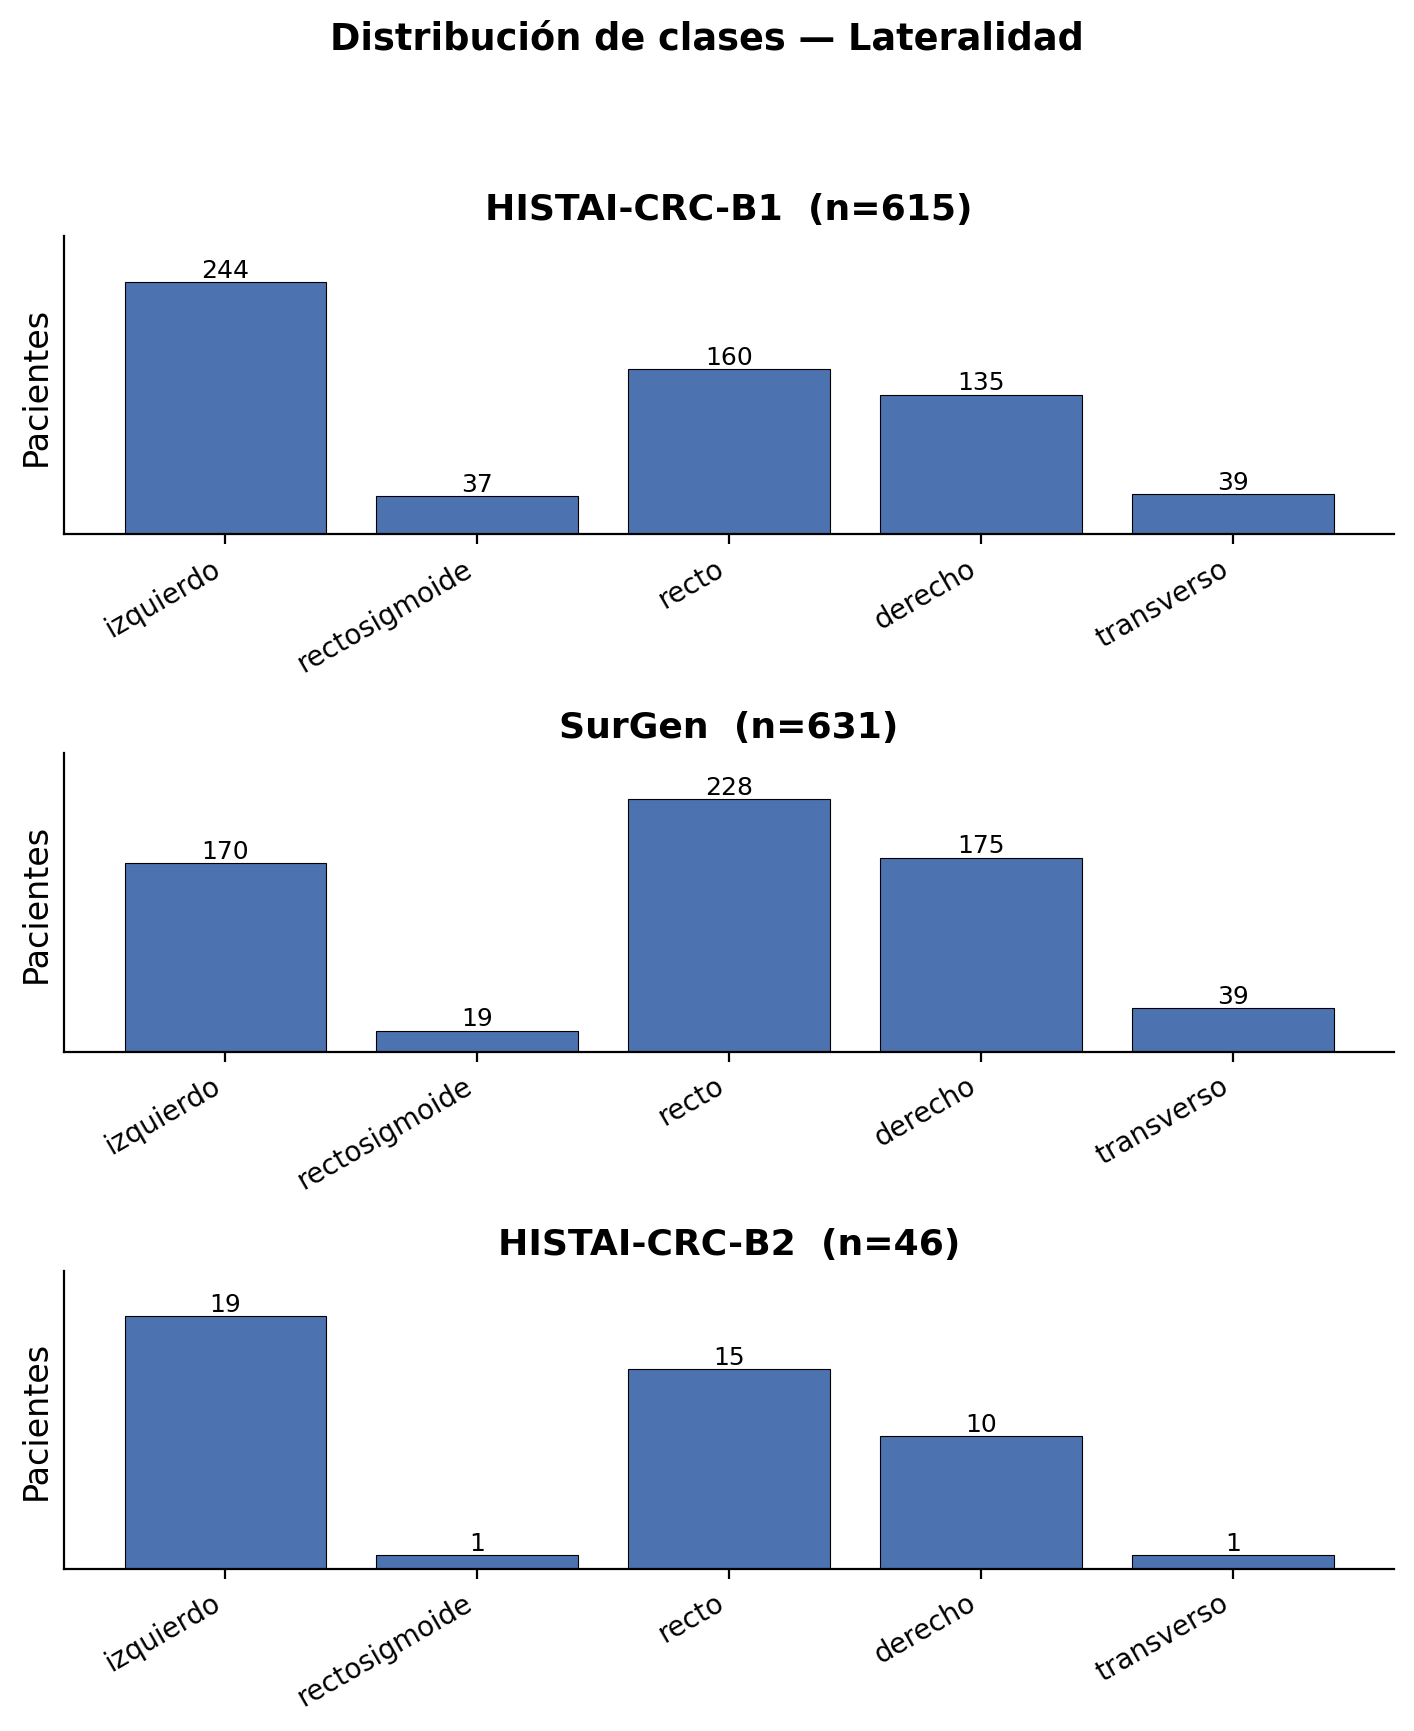
\includegraphics[width=0.72\textwidth]{figures/distribucion_clases/side}
\caption{Distribución de clases de la tarea Side por conjunto de datos.}
\label{fig:dist_side}
\end{figure}

\begin{figure}[htbp]
\centering
\begin{subfigure}[b]{0.3\textwidth}
\centering
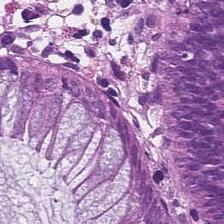
\includegraphics[width=\textwidth]{figures/ejemplos_clase/parches/side_izquierdo}
\caption{Izquierdo}
\end{subfigure}\hfill
\begin{subfigure}[b]{0.3\textwidth}
\centering
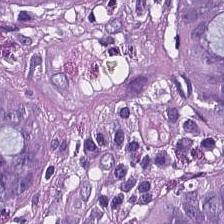
\includegraphics[width=\textwidth]{figures/ejemplos_clase/parches/side_rectosigmoide}
\caption{Rectosigmoide}
\end{subfigure}\hfill
\begin{subfigure}[b]{0.3\textwidth}
\centering
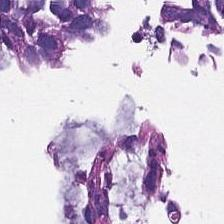
\includegraphics[width=\textwidth]{figures/ejemplos_clase/parches/side_recto}
\caption{Recto}
\end{subfigure}
\\[2ex]
\begin{minipage}{0.62\textwidth}
\centering
\begin{subfigure}[b]{0.48\textwidth}
\centering
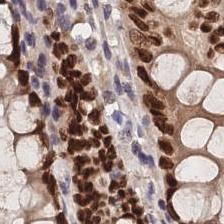
\includegraphics[width=\textwidth]{figures/ejemplos_clase/parches/side_derecho}
\caption{Derecho}
\end{subfigure}\hfill
\begin{subfigure}[b]{0.48\textwidth}
\centering
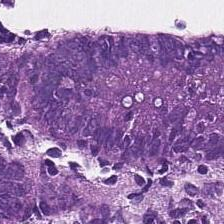
\includegraphics[width=\textwidth]{figures/ejemplos_clase/parches/side_transverso}
\caption{Transverso}
\end{subfigure}
\end{minipage}
\caption{Ejemplos representativos de parches para cada clase de Side.}
\label{fig:ejemplos_side}
\end{figure}

La Figura~\ref{fig:ejemplos_side} presenta ejemplos representativos de parches asociados a las categorías de lateralidad. Estas imágenes ilustran la variabilidad visual de las muestras.

\subsubsection{Desempeño por modelo y dataset}

La tarea T4-SIDE comprende cinco categorías, por lo que el nivel de referencia uniforme para la \textit{balanced accuracy} corresponde a 0.2. En SurGen, UNI2 alcanza el mayor desempeño, con una \textit{balanced accuracy} de 0.372 y un IC 95\% de [0.329, 0.415]. Virchow2, Phikon-v2 y Prov-GigaPath obtienen valores de 0.339, 0.321 y 0.318, respectivamente. En HISTAI-CRC-B1, los resultados varían entre 0.293 para Phikon-v2 y 0.331 para Prov-GigaPath. Por tanto, las dos cohortes de mayor tamaño presentan desempeño por sobre el nivel de referencia, aunque con una utilidad predictiva todavía moderada.

En HISTAI-CRC-B2, los cuatro modelos obtienen valores entre 0.115 y 0.174, inferiores al nivel de referencia de 0.2. Sin embargo, esta cohorte contiene solo 46 pacientes y dos categorías poseen un único caso cada una. En consecuencia, la \textit{balanced accuracy} y las sensibilidades por clase tienen una elevada variabilidad, por lo que estos resultados no permiten establecer un ordenamiento confiable entre modelos.

El análisis por clase muestra diferencias relevantes entre cohortes. En HISTAI-CRC-B1, la categoría izquierdo presenta sensibilidades entre 0.607 y 0.660, mientras que la categoría derecho alcanza valores entre 0.481 y 0.519. En SurGen, recto es la categoría mejor detectada, con sensibilidades entre 0.675 y 0.737, seguida de derecho, con valores entre 0.434 y 0.560. En cambio, transverso y rectosigmoide presentan sensibilidades bajas en las cohortes evaluadas, coherentes con su representación limitada.

\begin{figure}[htbp]
\centering
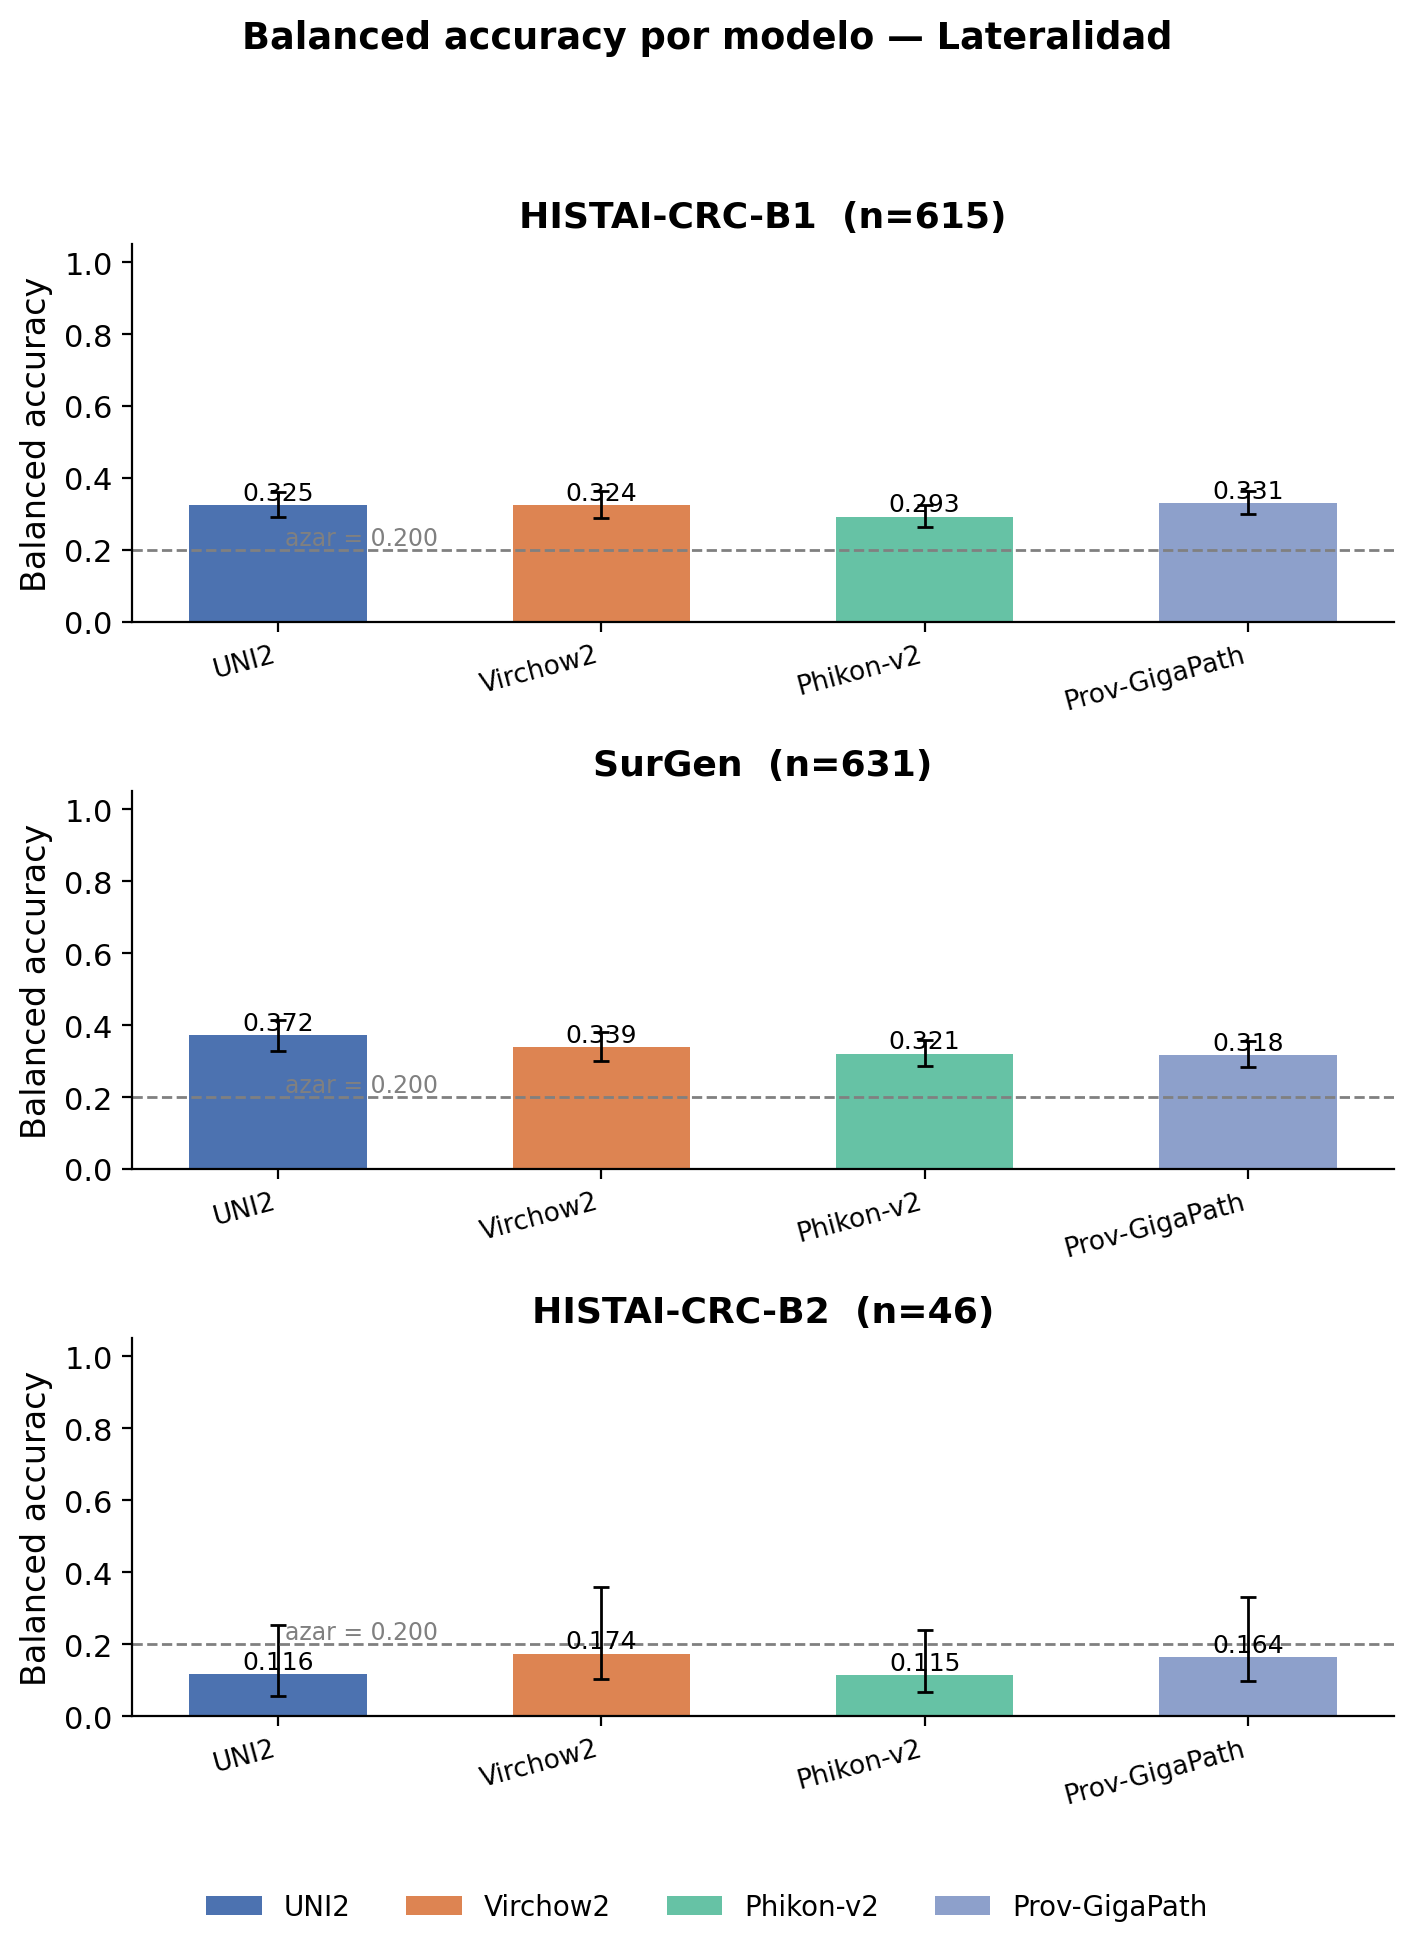
\includegraphics[width=0.72\textwidth]{figures/balanced_accuracy/side}
\caption{Balanced accuracy por modelo y conjunto de datos en la tarea Side. Barras de error: IC 95\% bootstrap.}
\label{fig:ba_side}
\end{figure}


Los valores numéricos completos se presentan en las
Tablas~\ref{tab:anexo_side_utilidad}; \ref{tab:anexo_side_sensibilidad}--\ref{tab:anexo_side_sensibilidad_surgen};
\ref{tab:anexo_side_fairness_edad}--\ref{tab:anexo_side_fairness_edad_surgen};
\ref{tab:anexo_side_fairness_sexo}--\ref{tab:anexo_side_fairness_sexo_surgen}; y
\ref{tab:anexo_side_crossdataset} (Apéndice~\ref{anexo:resultados_completos}).

\subsubsection{Equidad entre subgrupos}

En HISTAI-CRC-B1, las brechas por edad varían entre 0.028 y 0.074. En SurGen, estas oscilan entre 0.011 y 0.115, siendo Phikon-v2 el modelo con mayor diferencia por edad y Prov-GigaPath el de menor diferencia. Las brechas por sexo en las cohortes de mayor tamaño también son acotadas, con valores entre 0.032 y 0.061 en HISTAI-CRC-B1 y entre 0.024 y 0.057 en SurGen. La dirección de las diferencias cambia entre modelos, por lo que no se identifica un grupo de edad o sexo favorecido de manera consistente.

En HISTAI-CRC-B2, los grupos de edad de 50 a 70 años y de $\geq 70$ años incluyen $n=21$ y $n=22$ pacientes, respectivamente. Las brechas por edad varían entre 0.076 y 0.193. Por sexo, la cohorte incluye $n=26$ mujeres y $n=20$ hombres. Las brechas varían entre 0.136 y 0.306; Prov-GigaPath presenta la diferencia más alta, con \textit{balanced accuracy} de 0.373 en mujeres y de 0.067 en hombres.

Las diferencias observadas en HISTAI-CRC-B2 deben interpretarse de manera exploratoria. La cohorte total es pequeña, las categorías rectosigmoide y transverso poseen un único caso, y la composición de clases puede diferir entre los subgrupos evaluados. En este contexto, una \textit{balanced accuracy} cercana a cero en un grupo no permite por sí sola concluir que exista sesgo por sexo o edad; se requiere una cohorte externa de mayor tamaño y con soporte suficiente por categoría para evaluar esa hipótesis.

\subsubsection{Generalización cross-dataset}

La transferencia entre las cohortes colorrectales muestra caídas relevantes de rendimiento. Cuando SurGen actúa como conjunto de entrenamiento, la transferencia hacia HISTAI-CRC-B1 reduce la \textit{balanced accuracy} entre 0.085 y 0.166, equivalentes a pérdidas relativas de 26.8\% a 46.0\%. En la dirección inversa, desde HISTAI-CRC-B1 hacia SurGen, las caídas varían entre 0.080 y 0.115, equivalentes a 24.6\% a 39.1\%.

La transferencia hacia HISTAI-CRC-B2 presenta mayor incertidumbre. UNI2 disminuye 0.145 y Virchow2 disminuye 0.205, mientras que Phikon-v2 y Prov-GigaPath presentan diferencias pequeñas o negativas. Dado que HISTAI-CRC-B2 contiene solo 46 pacientes y presenta categorías con soporte mínimo, estas diferencias no permiten comparar de forma confiable la robustez de los modelos frente a cambios de cohorte.

Cuando HISTAI-CRC-B2 se utiliza como fuente de entrenamiento, se observan nuevamente deltas negativos hacia HISTAI-CRC-B1. Al igual que en T1, T2 y T3, este patrón es compatible con una estimación ID inestable en una cohorte pequeña y con desempeño limitado. Por tanto, no debe interpretarse como una evidencia de mejor generalización externa. Los resultados completos se presentan en la Tabla~\ref{tab:anexo_side_crossdataset}.

% ---------------------------------------------------------------------
En conjunto, T4-SIDE presenta una utilidad predictiva mayor que T3-SITE en las cohortes colorrectales de mayor tamaño. Esta diferencia es compatible con una menor granularidad de la etiqueta, ya que T4 agrupa la localización tumoral en cinco categorías, mientras que T3 utiliza nueve categorías anatómicas. Sin embargo, esta comparación debe interpretarse con cautela, porque ambas tareas no necesariamente incluyen exactamente los mismos pacientes ni la misma distribución de clases.

Los resultados por clase muestran que las categorías anatómicas más representadas, como izquierdo, derecho y recto, concentran las sensibilidades más altas. Las categorías con menor soporte, particularmente transverso y rectosigmoide, mantienen sensibilidades bajas. Este patrón es compatible con una influencia conjunta de la prevalencia de clases, la heterogeneidad morfológica y la definición de las categorías anatómicas.

Respecto de la equidad, HISTAI-CRC-B1 y SurGen no muestran un patrón consistente de favorecimiento por edad o sexo entre modelos. No obstante, las brechas deben interpretarse junto con la utilidad predictiva global, que sigue siendo moderada. En HISTAI-CRC-B2, las diferencias por edad y sexo son exploratorias y no permiten confirmar ni descartar una disparidad real, debido al tamaño reducido de los subgrupos y al soporte insuficiente de varias categorías.
% ---------------------------------------------------------------------


\subsection{T5: Clasificación de órgano}
\label{sec:resultado_organ}

\subsubsection{Descripción de la tarea y distribución de clases}

La tarea T5-ORGAN clasifica el órgano de origen de cada paciente en dos categorías, mama y colorrectal. Integra las 3675 observaciones analíticas de las seis cohortes mediante una partición fija de 2625 pacientes para entrenamiento, 525 para validación y 525 para prueba, con una distribución de 53.7\% para mama y 46.3\% para colorrectal. La Figura~\ref{fig:dist_organ} presenta la distribución de clases.

Esta tarea debe interpretarse como un experimento auxiliar de separabilidad entre cohortes. Ninguno de los datasets incluidos contiene muestras de ambos órganos, por lo que la etiqueta de órgano está asociada al origen de la cohorte. En consecuencia, el clasificador puede utilizar tanto diferencias entre tejidos como señales técnicas o institucionales asociadas al dataset, tales como tinción, escáner, preparación de la muestra o composición clínica de la cohorte.

\begin{figure}[htbp]
\centering
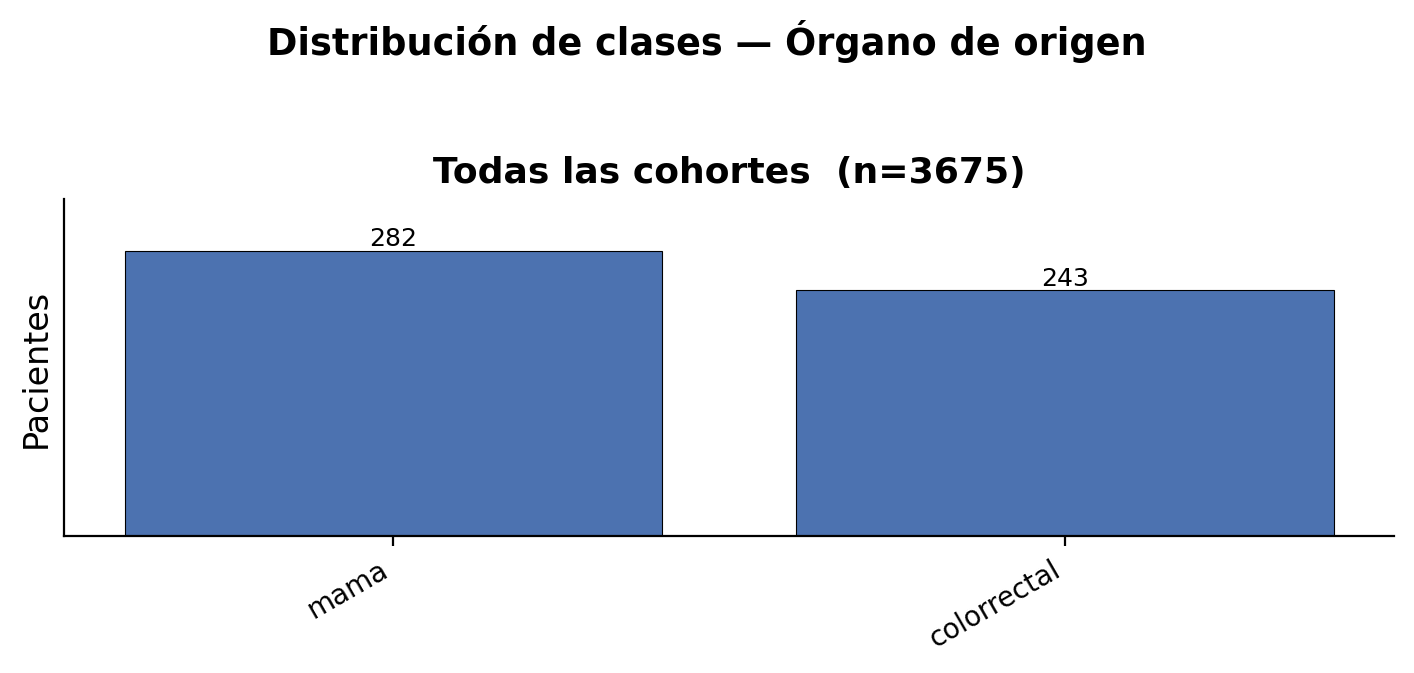
\includegraphics[width=\textwidth]{figures/distribucion_clases/organ}
\caption{Distribución de clases de la tarea Organ.}
\label{fig:dist_organ}
\end{figure}

\begin{figure}[htbp]
\centering
\begin{subfigure}[b]{0.45\textwidth}
\centering
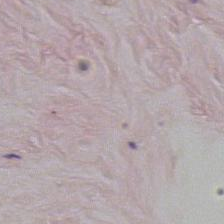
\includegraphics[width=\textwidth]{figures/ejemplos_clase/parches/organ_mama}
\caption{Mama}
\end{subfigure}\hfill
\begin{subfigure}[b]{0.45\textwidth}
\centering
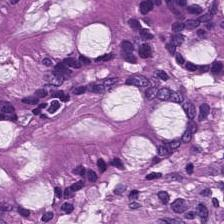
\includegraphics[width=\textwidth]{figures/ejemplos_clase/parches/organ_colorrectal}
\caption{Colorrectal}
\end{subfigure}
\caption{Ejemplos representativos de parches para cada clase de Organ.}
\label{fig:ejemplos_organ}
\end{figure}

La Figura~\ref{fig:ejemplos_organ} presenta ejemplos representativos de parches de mama y colorrectal. Estas imágenes ilustran diferencias visuales entre los dominios.

\subsubsection{Desempeño por modelo y dataset}

Los cuatro modelos resuelven T5-ORGAN con desempeño casi perfecto. La \textit{balanced accuracy} varía entre 0.996 para Prov-GigaPath y 1.000 para Virchow2; el AUC macro es 1.000 para los cuatro modelos. La sensibilidad para mama es 1.000 en todos los casos, mientras que la sensibilidad para colorrectal varía entre 0.992 y 1.000. Estos resultados muestran que las representaciones permiten separar casi perfectamente las observaciones de mama y colorrectal incluidas en este estudio.

Sin embargo, este desempeño no permite atribuir la separación exclusivamente a la morfología de los órganos. Como cada cohorte pertenece a un único órgano, la variable objetivo está confundida con el dataset de origen. Por ello, el clasificador puede estar aprovechando diferencias morfológicas entre mama y colorrectal, pero también firmas de adquisición, tinción, escáner, procesamiento de tejido, institución, composición clínica o procedimientos de curación de datos. T5-ORGAN demuestra separabilidad de las cohortes integradas, no una capacidad de clasificación de órgano independiente de esos factores.

\begin{figure}[htbp]
\centering
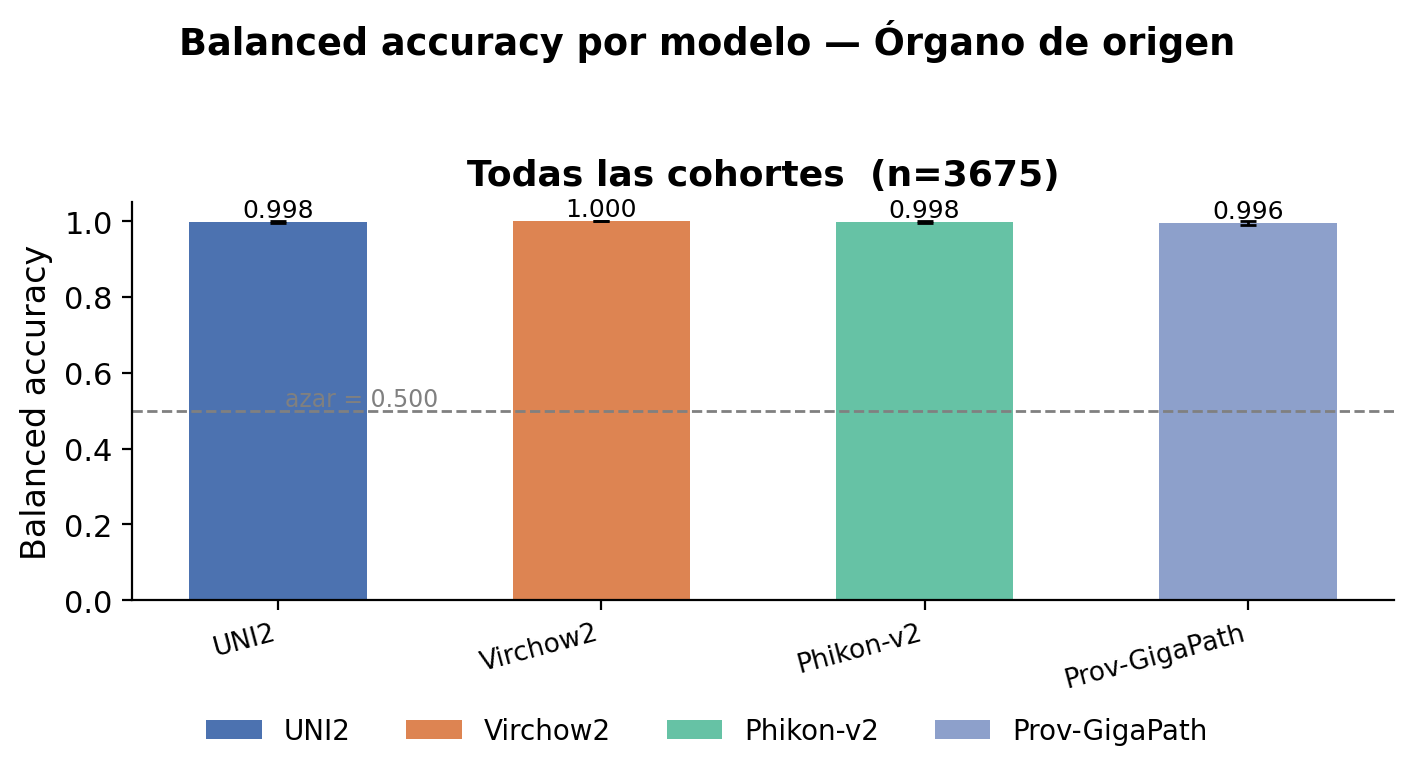
\includegraphics[width=\textwidth]{figures/balanced_accuracy/organ}
\caption{Balanced accuracy por modelo en la tarea Organ. Barras de error: IC 95\% bootstrap.}
\label{fig:ba_organ}
\end{figure}

Los valores numéricos completos se presentan en las
Tablas~\ref{tab:anexo_organ_utilidad}, \ref{tab:anexo_organ_sensibilidad} y
\ref{tab:anexo_organ_fairness} (Apéndice~\ref{anexo:resultados_completos}).

\subsubsection{Equidad entre subgrupos}
Las brechas de \textit{balanced accuracy} por edad se encuentran entre 0.000 y 0.010. Este resultado es consistente con la escasa cantidad de errores en la tarea, pero no debe interpretarse como evidencia suficiente de equidad algorítmica. Cuando el desempeño es prácticamente perfecto para todos los grupos, la brecha de rendimiento queda limitada por un efecto de techo y aporta poca información sobre la capacidad del modelo para mantener un desempeño equitativo en una tarea clínicamente más exigente.

La equidad por sexo no se evaluó, debido a la cobertura incompleta de esta variable en las cohortes integradas. Por tanto, T5-ORGAN no permite extraer conclusiones generales sobre equidad demográfica de los modelos fundacionales.

En conjunto, T5-ORGAN evidencia una separabilidad casi perfecta entre las observaciones de mama y colorrectal incluidas en las cohortes evaluadas. Este resultado es compatible con diferencias morfológicas importantes entre ambos órganos, pero no permite determinar cuánto del desempeño corresponde a dicha señal biológica y cuánto a características técnicas o institucionales asociadas al origen de los datos.

Por esta razón, T5 debe interpretarse como evidencia de confusión potencial entre la variable clínica y el dataset de origen. Sus brechas reducidas por edad reflejan principalmente el efecto de techo de una tarea casi perfectamente resuelta, y no constituyen una validación general de equidad. La sección siguiente evalúa de manera directa la separabilidad entre cohortes mediante clasificación de origen de dataset.


\subsection{Verificación experimental del \textit{center effect}}
\label{sec:verificacion_center_effect}

Con el fin de evaluar si los embeddings a nivel de paciente contienen señales asociadas al origen de las cohortes, se entrenó un clasificador cuyo objetivo es predecir el dataset de procedencia en lugar de la etiqueta clínica. Se reutilizó la configuración experimental del Capítulo~6: un clasificador MLP con 256 unidades ocultas y activación ReLU, $\alpha = 10^{-4}$, \texttt{max\_iter = 500}, sobremuestreo de las clases minoritarias y validación cruzada de 5 pliegues mediante \texttt{StratifiedGroupKFold}, agrupada por paciente y con \texttt{seed = 42}. Los intervalos de confianza del 95\% se obtuvieron mediante bootstrap no paramétrico de 1000 remuestreos a nivel de paciente.

El Experimento A evalúa la separabilidad entre datasets dentro de cada dominio clínico mediante clasificación de tres cohortes. El Experimento B compara pares de cohortes colorrectales. En particular, la comparación entre HISTAI-CRC-B1 e HISTAI-CRC-B2 permite evaluar la separabilidad entre cohortes que comparten escáner, mientras que las comparaciones que incluyen SurGen incorporan simultáneamente una diferencia de escáner y otros factores no controlados. Por ello, los resultados describen separabilidad entre cohortes, pero no permiten atribuir causalmente el desempeño a un único factor técnico o institucional.

En el Experimento A, el nivel de referencia para una clasificación uniforme de tres clases corresponde a $1/3 \approx 0{,}333$. En el Experimento B, que corresponde a clasificaciones binarias, el nivel de referencia es 0,5.

\begin{table}[htbp]
\centering
\caption{Resumen de la separabilidad entre cohortes mediante clasificación de origen de dataset. Los rangos de \textit{balanced accuracy} corresponden a los cuatro modelos fundacionales evaluados. El detalle completo se presenta en las Tablas~\ref{tab:anexo_center_effect_a} y \ref{tab:anexo_center_effect_b} del Apéndice~\ref{anexo:resultados_completos}.}
\label{tab:center_effect}
\small
\begin{tabular}{p{3.0cm} p{5.6cm} c c}
\toprule
\textbf{Dominio} & \textbf{Comparación} &
\textbf{$n_{\text{eval}}$} & \textbf{BA} \\
\midrule
Mama &
BCNB, HISTAI-Breast y HSI-BC &
1944 &
1.000 \\

Colorrectal &
SurGen, HISTAI-CRC-B1 e HISTAI-CRC-B2 &
1700 &
0.856 a 0.928 \\

Colorrectal &
HISTAI-CRC-B1 frente a HISTAI-CRC-B2, escáner compartido &
935 &
0.821 a 0.864 \\

Colorrectal &
SurGen frente a HISTAI-CRC-B1, escáner diferente &
1643 &
1.000 \\

Colorrectal &
SurGen frente a HISTAI-CRC-B2, escáner diferente &
822 &
1.000 \\
\bottomrule
\end{tabular}

\medskip
\footnotesize
\parbox{0.95\textwidth}{\textit{Nota:} La comparación de mama utiliza la cohorte común de 1944 pacientes disponible para los cuatro encoders, correspondiente a la cohorte analítica de T2-MOLSUB. Por ello, su tamaño difiere del reportado en T1-HER2.}
\end{table}

En el dominio de mama, las tres cohortes presentan una separabilidad prácticamente perfecta dentro de la cohorte común de 1944 pacientes utilizada en este experimento. Los cuatro modelos alcanzan una \textit{balanced accuracy} de 1.000 y un AUC de 1.000 para clasificar el dataset de origen. Este resultado muestra que los embeddings contienen una firma de cohorte muy marcada. Sin embargo, BCNB, HISTAI-Breast y HSI-BC difieren simultáneamente en institución, condiciones de adquisición, composición de pacientes, disponibilidad de metadatos y procesos de curación. Por tanto, esta comparación no permite atribuir la separación a un factor técnico o biológico específico.

El dominio colorrectal permite un contraste más informativo. HISTAI-CRC-B1 y HISTAI-CRC-B2 comparten el escáner Leica Aperio GT450 AT2, pero su origen sigue siendo altamente recuperable, con \textit{balanced accuracy} entre 0.821 y 0.864 y AUC entre 0.970 y 0.986. Esto muestra que existen diferencias entre cohortes que permanecen disponibles en las representaciones incluso cuando el escáner es compartido. Tales diferencias podrían estar asociadas a tinción, preparación y manejo del tejido, distribución clínica, anotación, calidad de las imágenes u otros factores no observados.

Las comparaciones entre SurGen y las cohortes HISTAI-CRC alcanzan una \textit{balanced accuracy} y un AUC de 1.000 en los cuatro modelos. Además, al clasificar conjuntamente SurGen, HISTAI-CRC-B1 e HISTAI-CRC-B2, los modelos alcanzan \textit{balanced accuracy} entre 0.856 y 0.928 y AUC entre 0.991 y 0.998. Estos resultados son compatibles con una alta separación entre las cohortes colorrectales y con diferencias adicionales de adquisición, incluido el uso de un escáner diferente en SurGen. Sin embargo, SurGen también puede diferir en múltiples factores no controlados. En consecuencia, la diferencia entre la separabilidad de B1 frente a B2 y la separabilidad perfecta de los pares que incluyen SurGen no permite cuantificar una contribución causal específica del escáner.

En conjunto, el experimento demuestra que el origen de la cohorte es altamente recuperable desde los embeddings evaluados. Este hallazgo es consistente con las caídas observadas en la generalización cross-dataset de T1 a T4 y refuerza la necesidad de interpretar tales caídas como el resultado potencial de múltiples fuentes de cambio de distribución. El diseño actual no permite determinar qué proporción corresponde a diferencias morfológicas reales, factores técnicos de adquisición o características institucionales y clínicas de las cohortes. El detalle completo de las métricas e intervalos de confianza se presenta en las Tablas~\ref{tab:anexo_center_effect_a} y \ref{tab:anexo_center_effect_b} del Apéndice~\ref{anexo:resultados_completos}.

\section{Conclusiones del capítulo}
\label{sec:sintesis_cap6}

Los resultados muestran que la utilidad predictiva depende principalmente de la tarea y de la cohorte evaluada. T2-MOLSUB presenta mayor capacidad discriminativa que T1-HER2 en BCNB, mientras que las tareas colorrectales reducen su desempeño al aumentar la granularidad de las categorías. T3-SITE representa el escenario de mayor complejidad, con ocho o nueve clases según la cohorte, mientras que T4-SIDE obtiene resultados comparativamente superiores al utilizar una definición anatómica menos granular. T5-ORGAN alcanza desempeño casi perfecto, pero debe interpretarse como una tarea de separabilidad entre cohortes y no como una validación aislada de clasificación morfológica de órgano.

La Tabla~\ref{tab:sintesis_utilidad_equidad} resume cualitativamente la utilidad predictiva, la estabilidad de las estimaciones de equidad y la generalización entre cohortes. Los colores representan la interpretabilidad de los resultados bajo las condiciones de evaluación y no una clasificación definitiva de equidad, inequidad o sesgo.

\begin{table}[htbp]
\centering
\caption{Síntesis cualitativa de utilidad predictiva, equidad y generalización por tarea y cohorte. Los colores representan la estabilidad e interpretabilidad de los resultados, no una clasificación definitiva de sesgo o equidad.}
\label{tab:sintesis_utilidad_equidad}
\small
\resizebox{\textwidth}{!}{%
\begin{tabular}{l l p{3.2cm} p{3.6cm} p{3.4cm}}
\toprule
\textbf{Tarea} &
\textbf{Cohorte} &
\textbf{Utilidad predictiva} &
\textbf{Equidad por subgrupos} &
\textbf{Generalización} \\
\midrule

T1-HER2 &
BCNB &
\cellcolor{yellow!25}Limitada &
\cellcolor{yellow!25}Brechas variables por edad &
\cellcolor{yellow!25}Caída moderada hacia HISTAI-Breast \\

T1-HER2 &
HISTAI-Breast &
\cellcolor{yellow!25}Limitada &
\cellcolor{green!20}Sin patrón etario consistente &
\cellcolor{yellow!25}Caída moderada hacia BCNB \\

T1-HER2 &
HSI-BC &
\cellcolor{red!25}Exploratoria, $n=44$ &
\cellcolor{red!25}No concluyente &
\cellcolor{red!25}No interpretable de forma estable \\
\midrule

T2-MOLSUB &
BCNB &
\cellcolor{green!20}Mayor utilidad en mama &
\cellcolor{yellow!25}Brechas variables por edad &
\cellcolor{yellow!25}Caída hacia cohortes externas \\

T2-MOLSUB &
HISTAI-Breast &
\cellcolor{yellow!25}Moderada &
\cellcolor{yellow!25}Brechas variables por edad &
\cellcolor{yellow!25}Caída desde BCNB \\

T2-MOLSUB &
HSI-BC &
\cellcolor{red!25}Exploratoria, $n=44$ &
\cellcolor{red!25}No concluyente &
\cellcolor{red!25}No interpretable de forma estable \\
\midrule

T3-SITE &
HISTAI-CRC-B1 &
\cellcolor{yellow!25}Moderada para nueve clases &
\cellcolor{green!20}Sin patrón consistente &
\cellcolor{yellow!25}Caída relevante hacia SurGen \\

T3-SITE &
SurGen &
\cellcolor{green!20}Mayor utilidad de T3 &
\cellcolor{green!20}Sin patrón consistente &
\cellcolor{yellow!25}Caída relevante hacia otras cohortes \\

T3-SITE &
HISTAI-CRC-B2 &
\cellcolor{red!25}Exploratoria, $n=57$ &
\cellcolor{red!25}No concluyente &
\cellcolor{red!25}No interpretable de forma estable \\
\midrule

T4-SIDE &
HISTAI-CRC-B1 &
\cellcolor{yellow!25}Moderada &
\cellcolor{green!20}Sin patrón consistente &
\cellcolor{yellow!25}Caída hacia SurGen \\

T4-SIDE &
SurGen &
\cellcolor{green!20}Mayor utilidad de T4 &
\cellcolor{yellow!25}Brechas variables por edad &
\cellcolor{yellow!25}Caída hacia HISTAI-CRC-B1 \\

T4-SIDE &
HISTAI-CRC-B2 &
\cellcolor{red!25}Exploratoria, $n=46$ &
\cellcolor{red!25}No concluyente &
\cellcolor{red!25}No interpretable de forma estable \\
\midrule

T5-ORGAN &
Cohorte combinada &
\cellcolor{blue!20}Casi perfecta, pero confundida &
\cellcolor{blue!20}Efecto de techo &
\cellcolor{blue!20}No aplica \\
\bottomrule
\end{tabular}%
}

\medskip
\footnotesize
\parbox{0.97\textwidth}{\textit{Nota:} Verde indica resultados relativamente estables y sin un patrón demográfico consistente entre modelos. Amarillo indica resultados interpretables con limitaciones de utilidad, variabilidad entre modelos o caída de generalización. Rojo indica resultados exploratorios, condicionados por tamaño muestral reducido o soporte insuficiente de clases y subgrupos. Azul indica una dimensión no evaluable, no aplicable o dominada por confusión estructural. Los colores no constituyen una clasificación definitiva de equidad, inequidad o sesgo.}
\end{table}

Las diferencias entre cohortes son más consistentes que las diferencias entre modelos fundacionales. BCNB, SurGen e HISTAI-CRC-B1 presentan resultados más estables, mientras que HSI-BC e HISTAI-CRC-B2 concentran la mayor incertidumbre debido a su tamaño reducido, la representación limitada de algunas clases y la menor estabilidad de las estimaciones. HISTAI-Breast presenta resultados intermedios, en un contexto donde la disponibilidad y trazabilidad de biomarcadores constituye una fuente adicional de incertidumbre. Ningún encoder domina de manera transversal en todas las tareas y cohortes.

Respecto de la equidad, no se identifica un patrón de favorecimiento por edad o sexo que sea consistente entre modelos y cohortes de mayor tamaño. Sin embargo, una brecha reducida no implica por sí sola equidad clínicamente satisfactoria, especialmente en tareas con utilidad predictiva limitada. Las estimaciones de HSI-BC e HISTAI-CRC-B2 deben considerarse exploratorias, ya que el tamaño de los subgrupos y el soporte de clases no permiten establecer conclusiones robustas sobre disparidad demográfica.

La generalización cross-dataset muestra caídas relevantes de desempeño y una dependencia marcada de la cohorte de entrenamiento y evaluación. El experimento de clasificación de origen de dataset refuerza esta observación: las cohortes son altamente separables desde los embeddings, incluso HISTAI-CRC-B1 e HISTAI-CRC-B2, que comparten escáner. Las comparaciones que incluyen SurGen alcanzan separabilidad perfecta, pero estas diferencias no permiten atribuir causalmente el resultado al escáner, ya que también intervienen factores de adquisición, institución, composición clínica, anotación y curación de datos. En conjunto, los resultados respaldan que la evaluación de modelos fundacionales en patología computacional debe considerar simultáneamente la tarea clínica, la calidad y representatividad de las cohortes, la estabilidad de las métricas de equidad y la generalización entre centros.